% \iffalse meta-comment
%
% Transformed from bookshelf.xml by ClassPack db2dtx.xsl
% version 1.19 (2020-05-19) on Saturday 23 May 2020 at 23:33:08
%
% bookshelf.dtx is copyright © 2020 by Peter Flynn <peter@silmaril.ie>
%
% This work may be distributed and/or modified under the
% conditions of the LaTeX Project Public License, either
% version 1.3 of this license or (at your option) any later
% version. The latest version of this license is in:
%
%     http://www.latex-project.org/lppl.txt
%
% and version 1.3 or later is part of all distributions of
% LaTeX version 2005/12/01 or later.
%
% This work has the LPPL maintenance status ‘maintained’.
% 
% The current maintainer of this work is Peter Flynn <peter@silmaril.ie>
%
% This work consists of the files bookshelf.dtx and bookshelf.ins,
% the derived file , 
% and any other ancillary files listed in the MANIFEST.
%
% \fi
% \iffalse
%<*driver>
\ProvidesFile{bookshelf.dtx}
%</driver>
%<class>\NeedsTeXFormat{LaTeX2e}[2017/04/15]
%<class>\ProvidesClass{bookshelf}[2020/05/24 v0.5
%<class>  Turn your bibliography into a bookshelf image]
%<*driver>
\RequirePackage{fix-cm}% included by default.
\PassOptionsToPackage{svgnames}{xcolor}% xcolor/dox/hyperref implied
\documentclass[12pt]{ltxdoc}
%%
%% Packages added for documentation
%%
\usepackage{dox}% used by default. (0)%
  \makeatletter
  \doxitem[idxtype=attribute]{Attribute}{CPK@attribute}{attributes}
  \makeatother
  \makeatletter
  \doxitem[idxtype=attributevalue]{AttributeValue}{CPK@attributevalue}{attribute values}
  \makeatother
  \makeatletter
  \doxitem[idxtype=class]{Class}{CPK@class}{classes}
  \makeatother
  \makeatletter
  \doxitem[idxtype=colour]{Colour}{CPK@colour}{colours}
  \makeatother
  \makeatletter
  \doxitem[idxtype=counter]{Counter}{CPK@counter}{counters}
  \makeatother
  \makeatletter
  \doxitem[idxtype=DTD]{DTD}{CPK@dtd}{DTDs/Schemas}
  \makeatother
  \makeatletter
  \doxitem[idxtype=element]{Element}{CPK@element}{element types}
  \makeatother
  \makeatletter
  \doxitem[idxtype=entity]{Entity}{CPK@entity}{entities}
  \makeatother
  \makeatletter
  \doxitem[idxtype=error]{Error}{CPK@error}{errors}
  \makeatother
  \makeatletter
  \doxitem[idxtype=field]{Field}{CPK@field}{fields}
  \makeatother
  \makeatletter
  \doxitem[idxtype=file]{File}{CPK@file}{files}
  \makeatother
  \makeatletter
  \doxitem[idxtype=font]{Font}{CPK@font}{fonts}
  \makeatother
  \makeatletter
  \doxitem[idxtype=function]{Function}{CPK@function}{functions}
  \makeatother
  \makeatletter
  \doxitem[idxtype=language]{Language}{CPK@language}{languages}
  \makeatother
  \makeatletter
  \doxitem[macrolike,idxtype=length]{Length}{CPK@length}{lengths}
  \makeatother
  \makeatletter
  \doxitem[idxtype=mode]{Mode}{CPK@mode}{modes}
  \makeatother
  \makeatletter
  \doxitem[idxtype=option]{Option}{CPK@option}{options}
  \makeatother
  \makeatletter
  \doxitem[idxtype=package]{Package}{CPK@package}{packages}
  \makeatother
  \makeatletter
  \doxitem[idxtype=variable]{Variable}{CPK@variable}{variables}
  \makeatother
  \makeatletter
  \doxitem[idxtype=parameter]{Parameter}{CPK@parameter}{parameters}
  \makeatother
  \makeatletter
  \doxitem[macrolike,idxtype=switch]{Switch}{CPK@switch}{switches}
  \makeatother
  \makeatletter
  \doxitem[idxtype=template]{Template}{CPK@template}{templates}
  \makeatother
  \makeatletter
  \doxitem[idxtype=typeface]{Typeface}{CPK@typeface}{typefaces}
  \makeatother
  \makeatletter
  \doxitem[macrolike,idxtype=box]{Box}{CPK@box}{boxes}
  \makeatother
  \newcommand{\LabelFont}[2][\relax]{\strut
    {\fontencoding\encodingdefault
	    \fontfamily{lmtt}\fontseries{lc}#1\selectfont#2}\space}
  \makeatletter
  \let\CPK@macro\macro\let\CPK@endmacro\endmacro
  \makeatother
  \makeatletter
  \let\CPK@environment\environment\let\CPK@endenvironment\endenvironment
  \makeatother
  \makeatletter
  \def\PrintAttributeName#1{\LabelFont{@#1}}
  \makeatother
  \def\PrintAttributeValueName#1{\LabelFont{"#1"}}
  \def\PrintClassName#1{\LabelFont[\fontfamily{lmss}]{#1}}
  \def\PrintColourName#1{\LabelFont[\color{#1}]{#1}}
  \def\PrintCounterName#1{\LabelFont{#1}}
  \def\PrintDTDName#1{\LabelFont{#1}}
  \def\PrintElementName#1{\LabelFont{<#1>}}
  \def\PrintEntityName#1{\LabelFont{\&#1;}}
  \def\PrintEnvironmentName#1{\LabelFont[\fontfamily{lmss}]{#1}}
  \def\PrintErrorName#1{\LabelFont[\color{Red}!]{#1}}
  \def\PrintFunctionName#1{\LabelFont[\bfseries\itshape]{#1}}
  \def\PrintLanguageName#1{\LabelFont{#1}}
  \def\PrintLengthName#1{\LabelFont{#1}}
  \def\PrintMacroName#1{\LabelFont{#1}}
  \def\PrintModeName#1{\LabelFont[\sffamily]{\textlangle#1\textrangle}}
  \def\PrintOptionName#1{\LabelFont[\bfseries]{#1}}
  \def\PrintPackageName#1{\LabelFont[\fontfamily{lmss}]{#1}}
  \def\PrintSwitchName#1{\LabelFont{#1}}
  \def\PrintTemplateName#1{\LabelFont[\bfseries]{#1}}
  \def\PrintVariableName#1{\LabelFont[\ttfamily]{#1}}
  \def\PrintParameterName#1{\LabelFont[\ttfamily]{#1}}
  \def\PrintFieldName#1{\LabelFont[\ttfamily]{#1}}
%% fontenc omit: conflict: fontspec (3)
%% inputenc omit: conflict: fontspec (6)
\usepackage{fontspec}% part/@conformance=xelatex detected. (7)%
  \renewcommand{\textsc}[1]{{\small\MakeTextUppercase{#1}}}
\usepackage{noto}% requested by author (15)%
\usepackage{luximono}% requested by author (16)%
\usepackage{mflogo}% used by default. (36)%
\usepackage[british]{babel}% used by default. (41)%
\usepackage[backend=biber,doi=true,
  isbn=true,url=true,uniquename=false,style=apa]{biblatex}% bibliography/@arch=biblatex detected. (42)%
  \makeatletter
  \AtBeginDocument{%
	    \setlength{\bibitemsep}{1ex}%
	    \setlength{\bibnamesep}{1.5\itemsep}%
	    \defbibheading{shortbib}[References]%
	      {\section{#1}}}
	  \@ifpackagewith{babel}{british}{%
	    \DeclareLanguageMapping{british}%
	      {british-apa}}{\relax}
  \makeatother
  \makeatletter
  \providetoggle{blx@skipbiblist}
  \makeatother
\usepackage{calc}% used by default. (50)%
  \makeatletter
  {\scriptsize
	    \global\advance\@totalleftmargin by1em
	    \global\advance\MacroIndent by.5em}
  \makeatother
\usepackage{ccaption}% used by default. (53)%
  \captionnamefont{\bfseries}
  \captionstyle{\raggedright}
\usepackage[inline]{enumitem}% use of 'variablelist' detected (57)%
  \setlist[description]{style=unboxed}
  \setlist[itemize]{leftmargin=2em}
  \setlist[enumerate]{leftmargin=2em}
  \newlist{inlineenum}{enumerate*}{1}
  \setlist[inlineenum,1]{label=\emph{\alph*}),
	    itemjoin={{; }},itemjoin*={{; and }}}
\usepackage{fancyhdr}% requested by author (59)%
  \makeatletter
  \pagestyle{fancy}
	    \cfoot{}
	    \lhead{\footnotesize\rightmark}
	    \rhead{\small\thepage}
	    \rfoot{\footnotesize The \LaTeX\
	      \textsf{\SIL@docname} \SIL@doctype}
	    \renewcommand{\headrulewidth}{0pt}
	    \renewcommand{\footrulewidth}{0pt}
  \makeatother
\usepackage{relsize}% use of 'acronym' detected (65)%
\usepackage{textcase}% used by default. (68)%
\usepackage{float}% used by default. (70)%
  \renewcommand{\topfraction}{.85}
  \renewcommand{\bottomfraction}{.7}
  \renewcommand{\textfraction}{.15}
  \renewcommand{\floatpagefraction}{.66}
  \renewcommand{\dbltopfraction}{.66}
  \renewcommand{\dblfloatpagefraction}{.66}
  \setcounter{topnumber}{9}
  \setcounter{bottomnumber}{9}
  \setcounter{totalnumber}{20}
  \setcounter{dbltopnumber}{9}
\usepackage[level]{fmtcount}% xref/@linkend➝listitem/xml:id detected. (71)%
\usepackage[a4paper,left=30mm,top=25mm,
  textwidth=150mm,textheight=225mm,headheight=15pt]{geometry}% used by default. (72)%
\usepackage{hypdoc}% requested by author (78)%
  \hypersetup{linkcolor=DarkBlue,urlcolor=Blue,citecolor=Red}
  \ExecuteBibliographyOptions{maxcitenames=1}
  \DeclareFieldFormat{citehyperref}{%
	    \DeclareFieldAlias{bibhyperref}{noformat}% Avoid nested links
	    \bibhyperref{#1}}
  \DeclareFieldFormat{textcitehyperref}{%
	    \DeclareFieldAlias{bibhyperref}{noformat}% Avoid nested links
	    \bibhyperref{%
	    #1%
	    \ifbool{cbx:parens}
	    {\bibcloseparen\global\boolfalse{cbx:parens}}
	    {}}}
  \savebibmacro{cite}
  \savebibmacro{textcite}
  \renewbibmacro*{cite}{%
	    \printtext[citehyperref]{%
	    \restorebibmacro{cite}%
	    \usebibmacro{cite}}}
  \renewbibmacro*{textcite}{%
	    \ifboolexpr{
	    ( not test {\iffieldundef{prenote}} and
	    test {\ifnumequal{\value{citecount}}{1}} )
	    or
	    ( not test {\iffieldundef{postnote}} and
	    test {\ifnumequal{\value{citecount}}{\value{citetotal}}} )
	    }
	    {\DeclareFieldAlias{textcitehyperref}{noformat}}
	    {}%
	    \printtext[textcitehyperref]{%
	    \restorebibmacro{textcite}%
	    \usebibmacro{textcite}}}
\usepackage{listings}% use of 'programlisting' detected (85)%
  \lstdefinelanguage{dummy}
	    {morekeywords={dummy}}
  \lstdefinelanguage{Makefile}
	  {otherkeywords={.PHONY,.DEFAULT},%
	    morekeywords={PHONY,DEFAULT,shell,ifeq,else,endif},%
	    keywordsprefix={.},%
	    moredelim=[l][\color{Green}]{:},%
	    morecomment=[l]{\#},%
	    moredelim=[s][\color{Blue}]{\$(}{)}%
	  }
  \lstdefinelanguage{DocBook}[]{XML}
	    {morekeywords={abstract,address,affiliation,annotation,arg,
	    author,book,chapter,classname,cmdsynopsis,command,
	    constraintdef,contrib,copyright,cover,date,email,emphasis,
	    envar,filename,firstname,footnote,guibutton,guilabel,
	    guimenu,guimenuitem,guisubmenu,holder,info,itemizedlist,
	    listitem,literal,member,option,orderedlist,orgdiv,orgname,
	    package,para,parameter,part,personname,phrase,procedure,
	    productname,programlisting,quote,refsection,remark,
	    constructorsynopsis,methodparan,modifier,funcparams,olink,
	    bibliography,biblioentry,biblioset,subtitle,artpagenums,
	    volumenum,issuenum,DOCTYPE,SYSTEM,xml:id,releaseinfo,
	    replaceable,revdescription,revhistory,revision,sect1,sect2,
	    sect3,sect4,seg,seglistitem,segmentedlist,segtitle,
	    simplelist,step,surname,systemitem,tag,term,title,uri,
	    userinput,variablelist,varlistentry,wordasword,xref,year,
	    xlink:href}}
	  
  \makeatletter
  \lstdefinelanguage{bash}
	    {morestring=[s]{[]},morekeywords={exit,logout,yes,no,@,
	    password,ssh,URL,cd,dvips,latex,ls,makeindex,man,mkdir,
	    pdflatex,sudo,texconfig,texdoc,updmap,xelatex,biber,
	    latexmk,bibtex}} 
	  
  \makeatother
  \lstdefinelanguage{APA}[]{XML}
	    {morekeywords={TTL}}
	  
  \lstdefinelanguage{OOXML}[]{XML}
	    {morekeywords={w:p,w:pPr,w:pStyle,w:rPr,w:rFonts,
	    w:r,w:t,w:lang}}
	  
  \lstdefinelanguage{SGML}[]{XML}
	    {morekeywords={sec,ttl}}
	  
  \lstdefinelanguage{DTD}[]{XML}
	    {morekeywords={ELEMENT,ENTITY,ATTLIST,CDATA,ID,REQUIRED,
	    IMPLIED,PCDATA}}
	  
  \lstdefinelanguage{Runoff}
	    {morekeywords={h1}}
	  
  \lstdefinelanguage{GML}
	    {morekeywords={h1}}
	  
  \lstdefinelanguage{Scribe}
	    {morekeywords={Heading},morestring=[s]{[]}}
	  
  \lstdefinelanguage{RTF}[]{TeX}
	    {moretexcs={rtf,ansi,deff,adeflang,fonttbl,f,froman,fprq,
	    fcharset,f1,fswiss,falt,fnil,colortbl,red,green,blue,
	    stylesheet,s,snext,nowidctlpar,hyphen,hyphlead,hyphtrail,
	    hyphmax,cf,kerning,dbch,af,langfe,afs,alang,loch,fs,
	    pgndec,pard,plain,qc,sb,sa,keepn,b,ab,rtlch,ltrch,par}}

  \lstdefinelanguage{TEI}[]{XML}
	    {morekeywords={TEI,TEI.2,teiHeader,fileDesc,sourceDesc,
	    titleStmt,title,author,editor,respStmt,resp,name,
	    editionStmt,edition,text,body,publicationStmt,publisher,
	    div,div1,placeName,lg,l,s,cl,phr,w,list,distinct,p,pb,
	    mls,div2,head,num,val,app,lem,rdg,q,sup,uncl,note,
	    DOCTYPE,SYSTEM,xml:id}}[keywords,comments,strings]
	  
  \lstdefinelanguage{XSLT2}[]{XML}
	    {morekeywords={xsl:stylesheet,xsl:transform,
	    xsl:apply-imports,xsl:attribute-set,xsl:decimal-format,
	    xsl:import,xsl:include,xsl:key,xsl:namespace-alias,
	    xsl:output,xsl:param,
	    xsl:preserve-space,xsl:strip-space,xsl:template,
	    xsl:variable,xsl:character-map,xsl:function,
	    xsl:import-schema,xsl:param,xsl:variable,
	    xsl:apply-imports,xsl:apply-templates,xsl:attribute,
	    xsl:call-template,xsl:choose,xsl:comment,xsl:copy,
	    xsl:copy-of,xsl:element,xsl:fallback,xsl:for-each,
	    xsl:if,xsl:message,xsl:number,xsl:otherwise,
	    xsl:processing-instruction,xsl:text,xsl:value-of,
	    xsl:variable,xsl:when,xsl:with-param,xsl:sort,
	    xsl:for-each-group,xsl:next-match,xsl:analyze-string,
	    xsl:namespace,xsl:result-document,xsl:copy,
	    xsl:fallback,xsl:document,xsl:sequence,
	    xsl:matching-substring,xsl:non-matching-substring,
	    xsl:perform-sort,xsl:output-character},
	    alsodigit={-}}
	  
  \lstdefinelanguage{LaTeXe}[LaTeX]{TeX}
	    {morekeywords = {selectlanguage,foreignlanguage,
	    textbrokenbar,textlangle,textrangle,subsection,url,
	    chapter,tableofcontents,part,subsubsection,paragraph,
	    subparagraph,maketitle,setlength,listoffigures,
	    listoftables,color,arraybackslash,includegraphics,
	    textcite,parencite,graphicspath,lstinline,
	    DeclareLanguageMapping,textcolor,definecolor,colorbox,
	    fcolorbox,RequirePackage,PassOptionsToPackage}}
	  
  \lstdefinelanguage{BIBTeX}{
	    morekeywords = {title,author,edition,publisher,year,
	    address},
	    morestring=[b]",
	    }
	  
  \lstdefinelanguage{Email}{
	    morekeywords={From,Subject,To,Date},
	    }
	  
  \lstset{defaultdialect=LaTeXe,frame=single,
	    framesep=.5em,backgroundcolor=\color{AliceBlue},
	    rulecolor=\color{LightSteelBlue},framerule=1pt}
	  
  \lstloadlanguages{LaTeXe,DocBook,XML,XSLT2,bash}
  \lstdefinelanguage{XMLFRAG}{tag=**[s]<>}[html]
  \lstnewenvironment{listingsdoc}
	    {\lstset{language={[LaTeX]TeX}}}
	    {}
  \newcommand\basicdefault[1]{\footnotesize
	    \color{Black}\ttfamily#1}
	  
  \lstset{basicstyle=\basicdefault{\spaceskip.5em}}
  \lstset{literate=
	    {§}{{\S}}1
	    {©}{{\raisebox{.125ex}{\copyright}\enspace}}1
	    {«}{{\guillemotleft}}1
	    {»}{{\guillemotright}}1
	    {Á}{{\'A}}1
	    {Ä}{{\"A}}1
	    {É}{{\'E}}1
	    {Í}{{\'I}}1
	    {Ó}{{\'O}}1
	    {Ö}{{\"O}}1
	    {Ú}{{\'U}}1
	    {Ü}{{\"U}}1
	    {ß}{{\ss}}2
	    {à}{{\`a}}1
	    {á}{{\'a}}1
	    {ä}{{\"a}}1
	    {é}{{\'e}}1
	    {í}{{\'i}}1
	    {ó}{{\'o}}1
	    {ö}{{\"o}}1
	    {ú}{{\'u}}1
	    {ü}{{\"u}}1
	    {¹}{{\textsuperscript1}}1
            {²}{{\textsuperscript2}}1
            {³}{{\textsuperscript3}}1
	    {ı}{{\i}}1
	    {—}{{---}}1
	    {’}{{'}}1
	    {…}{{\dots}}1
	    {➝}{{$leftarrow$}}1
            {⮠}{{$\hookleftarrow$}}1
	    {␣}{{\textvisiblespace}}1,
	    keywordstyle=\color{DarkGreen}\bfseries,
	    identifierstyle=\color{DarkRed},
	    commentstyle=\color{Gray}\upshape,
	    stringstyle=\color{DarkBlue}\upshape,
	    emphstyle=\color{Chocolate}\upshape,
	    showstringspaces=false,
	    columns=fullflexible,
	    keepspaces=true}
\usepackage{makeidx}% used by default. (87)%
  \makeindex
\usepackage{nicefrac}% used by default. (93)%
  \def\textonehalf{\ensuremath{\nicefrac12}}
\usepackage{parskip}% requested by author (95)%
\usepackage{sectsty}% requested by author (99)%
  \allsectionsfont{\sffamily\raggedright}
  \renewcommand*{\descriptionlabel}[1]{\hspace\labelsep
	    \sffamily\bfseries #1}
\usepackage[normalem]{ulem}% use of 'link' detected (105)%
\usepackage{url}% use of 'uri' detected (106)%
  \AtBeginDocument{\urlstyle{tt}}
\usepackage{varioref}% use of 'xref' detected (109)%
  \vrefwarning
  \labelformat{appendix}{Appendix~#1}
  \makeatletter
  \labelformat{chapter}{\@chapapp~#1}
  \makeatother
  \labelformat{section}{section~#1}
  \labelformat{subsection}{section~#1}
  \labelformat{subsubsection}{section~#1}
  \labelformat{paragraph}{section~#1}
  \labelformat{figure}{Figure~#1}
  \labelformat{table}{Table~#1}
  \labelformat{item}{item~#1}
  \renewcommand{\reftextcurrent}{elsewhere on this
	    page}
  \def\reftextafter{on the
	    \reftextvario{next}{following} page}
\usepackage{xcolor}% used by default. (117)%
  \makeatletter
  \@ifundefined{T}{%
	    \newcommand{\T}[2]{{\fontencoding{T1}%
	      \selectfont#2}}}{}
  \makeatother
\usepackage{classpack}[2020/05/19]% used by default. (122)%
\makeatletter
\newcommand{\SIL@doctype}{class}
\newcommand{\SIL@docname}{bookshelf}
\newcommand{\SIL@docowner}{Silmaril}
\makeatother
\addbibresource{bookshelf.bib}
\allsectionsfont{\sffamily}
%
%%
%% Settings for docstrip and ltxdoc 
%%
\EnableCrossrefs
\CodelineIndex
\RecordChanges
\begin{document}\raggedright
  \DocInput{bookshelf.dtx}
\end{document}
%</driver>
% \fi
%
% \CheckSum{718}
%
% \CharacterTable
%  {Upper-case    \A\B\C\D\E\F\G\H\I\J\K\L\M\N\O\P\Q\R\S\T\U\V\W\X\Y\Z
%   Lower-case    \a\b\c\d\e\f\g\h\i\j\k\l\m\n\o\p\q\r\s\t\u\v\w\x\y\z
%   Digits        \0\1\2\3\4\5\6\7\8\9
%   Exclamation   \!  Double quote  \"  Hash (number) \#
%   Dollar        \$  Percent       \%  Ampersand     \&
%   Acute accent  \'  Left paren    \(  Right paren   \)
%   Asterisk      \*  Plus          \+  Comma         \,
%   Minus         \-  Point         \.  Solidus       \/
%   Colon         \:  Semicolon     \;  Less than     \<
%   Equals        \=  Greater than  \>  Question mark \?
%   Commercial at \@  Left bracket  \[  Backslash     \\
%   Right bracket \]  Circumflex    \^  Underscore    \_
%   Grave accent  \`  Left brace    \{  Vertical bar  \|
%   Right brace   \}  Tilde         \~}
% 
% \changes{v0.5}{2020/05/24}{Finished initial testing: Replaced hyperref with hypdoc to avoid makeindex bug.}
% \changes{v0.4}{2020/05/19}{Completed documentation: 1) Updated note on bug in biber when processing sgml.bib; 2) Removed sgml.bib as example until problems are resolved; 3) Backtracked on attempt to use the monographic title for articles, chapters, etc; 4) Revised notes on production.}
% \changes{v0.3}{2020/05/14}{Finished first pass on documentation: 1) Done preliminary testing; 2) Script adapted for Mac OS X.}
% \changes{v0.2}{2020/05/12}{Started documentation: Code doc done, user doc still missing.}
% \changes{v0.1}{2020/05/7}{First packaged draft: Done manually from .tex file.}
%
% \GetFileInfo{bookshelf.dtx}
%
% \DoNotIndex{\@,\@@par,\@beginparpenalty,\@empty}
% \DoNotIndex{\@flushglue,\@gobble,\@input,\@makefnmark}
% \DoNotIndex{\@makeother,\@maketitle,\@namedef,\@ne}
% \DoNotIndex{\@spaces,\@tempa,\@tempb,\@tempswafalse}
% \DoNotIndex{\@tempswatrue,\@thanks,\@thefnmark,\@topnum}
% \DoNotIndex{\@@,\@elt,\@forloop,\@fortmp,\@gtempa}
% \DoNotIndex{\@totalleftmargin,\",\/,\@ifundefined,\@nil}
% \DoNotIndex{\@verbatim,\@vobeyspaces,\|,\~,\ ,\active}
% \DoNotIndex{\advance,\aftergroup,\begingroup,\bgroup}
% \DoNotIndex{\mathcal,\csname,\def,\documentstyle}
% \DoNotIndex{\dospecials,\edef,\egroup,\else,\endcsname}
% \DoNotIndex{\endgroup,\endinput,\endtrivlist}
% \DoNotIndex{\expandafter,\fi,\fnsymbol,\futurelet,\gdef}
% \DoNotIndex{\global,\hbox,\hss,\if,\if@inlabel}
% \DoNotIndex{\if@tempswa,\if@twocolumn,\ifcase,\ifcat}
% \DoNotIndex{\iffalse,\ifx,\ignorespaces,\index,\input}
% \DoNotIndex{\item,\jobname,\kern,\leavevmode,\leftskip}
% \DoNotIndex{\let,\llap,\lower,\m@ne,\next,\newpage}
% \DoNotIndex{\nobreak,\noexpand,\nonfrenchspacing}
% \DoNotIndex{\obeylines,\or,\protect,\raggedleft}
% \DoNotIndex{\rightskip,\rm,\sc,\setbox,\setcounter}
% \DoNotIndex{\small,\space,\string,\strut,\strutbox}
% \DoNotIndex{\thefootnote,\thispagestyle,\topmargin}
% \DoNotIndex{\trivlist,\tt,\twocolumn,\typeout,\vss,\vtop}
% \DoNotIndex{\xdef,\z@,\,,\@bsphack,\@esphack,\@noligs}
% \DoNotIndex{\@vobeyspaces,\@xverbatim,\`,\catcode,\end}
% \DoNotIndex{\escapechar,\frenchspacing,\glossary}
% \DoNotIndex{\hangindent,\hfil,\hfill,\hskip,\hspace,\ht}
% \DoNotIndex{\it,\langle,\leaders,\long,\makelabel}
% \DoNotIndex{\marginpar,\markboth,\mathcode,\mathsurround}
% \DoNotIndex{\mbox,\newcount,\newdimen,\newskip}
% \DoNotIndex{\nopagebreak,\parfillskip,\parindent}
% \DoNotIndex{\parskip,\penalty,\raise,\rangle,\section}
% \DoNotIndex{\setlength,\TeX,\topsep,\underline,\unskip}
% \DoNotIndex{\verb,\vskip,\vspace,\widetilde,\\,\%,\@date}
% \DoNotIndex{\@defpar,\[,\{,\},\],\count@,\ifnum,\loop}
% \DoNotIndex{\today,\uppercase,\uccode,\baselineskip}
% \DoNotIndex{\begin,\tw@,\a,\b,\c,\d,\e,\f,\g,\h,\i,\j,\k}
% \DoNotIndex{\l,\m,\n,\o,\p,\q,\r,\s,\t,\u,\v,\w,\x,\y,\z}
% \DoNotIndex{\A,\B,\C,\D,\E,\F,\G,\H,\I,\J,\K,\L,\M,\N,\O}
% \DoNotIndex{\P,\Q,\R,\S,\T,\U,\V,\W,\X,\Y,\Z,\1,\2,\3,\4}
% \DoNotIndex{\5,\6,\7,\8,\9,\0,\!,\#,\$,\&,\',\(,\)}
% \DoNotIndex{\+,\.,\:,\;,\<,\=,\>,\?,\_,\discretionary}
% \DoNotIndex{\immediate,\makeatletter,\makeatother}
% \DoNotIndex{\meaning,\newenvironment,\par,\relax}
% \DoNotIndex{\renewenvironment,\repeat,\scriptsize}
% \DoNotIndex{\selectfont,\the,\undefined,\arabic,\do}
% \DoNotIndex{\makeindex,\null,\number,\show,\write,\@ehc}
% \DoNotIndex{\@author,\@ehc,\@ifstar,\@sanitize,\@title}
% \DoNotIndex{\everypar,\if@minipage,\if@restonecol,\ifeof}
% \DoNotIndex{\ifmmode,\lccode,\newtoks,\onecolumn,\openin}
% \DoNotIndex{\p@,\SelfDocumenting,\settowidth}
% \DoNotIndex{\@resetonecoltrue,\@resetonecolfalse,\bf}
% \DoNotIndex{\clearpage,\closein,\lowercase,\@tempdima}
% \DoNotIndex{\@inlabelfalse,\selectfont,\mathcode}
% \DoNotIndex{\newmathalphabet,\rmdefault,\bfdefault}
% \DoNotIndex{\DeclareRobustCommand,\@ifpackagewith}
% \DoNotIndex{\SIL@doctype}
% \DoNotIndex{\SIL@docname}
% \DoNotIndex{\SIL@docowner}
% \DoNotIndex{\SIL@svgcolname}
% \DoNotIndex{\ifcase}
% \DoNotIndex{\SIL@svgcolval}
% \DoNotIndex{\addbibresource}
% \DoNotIndex{\immediate}
% \DoNotIndex{\input}
% \DoNotIndex{\documentclass}
% \DoNotIndex{\pagewidth}
% \DoNotIndex{\raggedright}
% \DoNotIndex{\name}
% \DoNotIndex{\SIL@topauthor}
% \DoNotIndex{\SIL@titleoneline}
% \DoNotIndex{\makebook}
% \DoNotIndex{\SILmfont}
% \DoNotIndex{\SILmfontname}
% \DoNotIndex{\vbox}
% \DoNotIndex{\fcolorbox}
% \DoNotIndex{\scalebox}
% \setcounter{tocdepth}{5}
% \setcounter{secnumdepth}{5}
% \makeatletter
% \def\@@doxdescribe#1#2{\endgroup \ifdox@noprint\else\marginpar{\raggedleft \textcolor{DarkRed}{\@nameuse{PrintDescribe#1}{#2}}}\fi \ifdox@noindex\else\@nameuse{Special#1Index}{#2}\fi \endgroup\@esphack\ignorespaces}
% \makeatother
%
% \def\fileversion{0.5}
% \def\filedate{2020/05/24}
% \title{The  \textsf{bookshelf} \LaTeXe\ document class\thanks{%
% This document corresponds to \textsf{bookshelf}
% \textit{v.}\ \fileversion $\beta$, dated \filedate.}
% \\[1em]\Large 
% Turn your bibliography into a bookshelf image}
% \author{Peter Flynn\\\normalsize Silmaril Consultants\\[-.25ex]\normalsize Instant Textual Gratification Division\\\normalsize(\url{peter@silmaril.ie})}
% \maketitle
% \renewcommand{\abstractname}{Summary}\thispagestyle{empty}
% \begin{abstract}
% \parskip=0.5\baselineskip
% \advance\parskip by 0pt plus 2pt
% \parindent=0pt% \noindent
% The \textsf{bookshelf} package uses
% \textsf{biblatex} and
% \emph{biber} to turn a \BibTeX{}
% bibliography file into a randomly-coloured, randomly-sized
% shelf of books, with the title and author in a randomly-chosen
% typeface. The image (converted to {\smaller JPEG} from
% {\smaller PDF}) can then be used as a background in
% \emph{Zoom},
% \emph{Teams},
% \emph{WhatsApp} etc video calls. It
% requires a little preliminary work with the supplied script to
% set up a list of all your fonts, a list of colors, and a list
% of the \BibTeX{} entry names in your {\ttfamily{}.bib}
% file, but otherwise should work on any modern \TeX{}
% distribution.\par
% \par\centering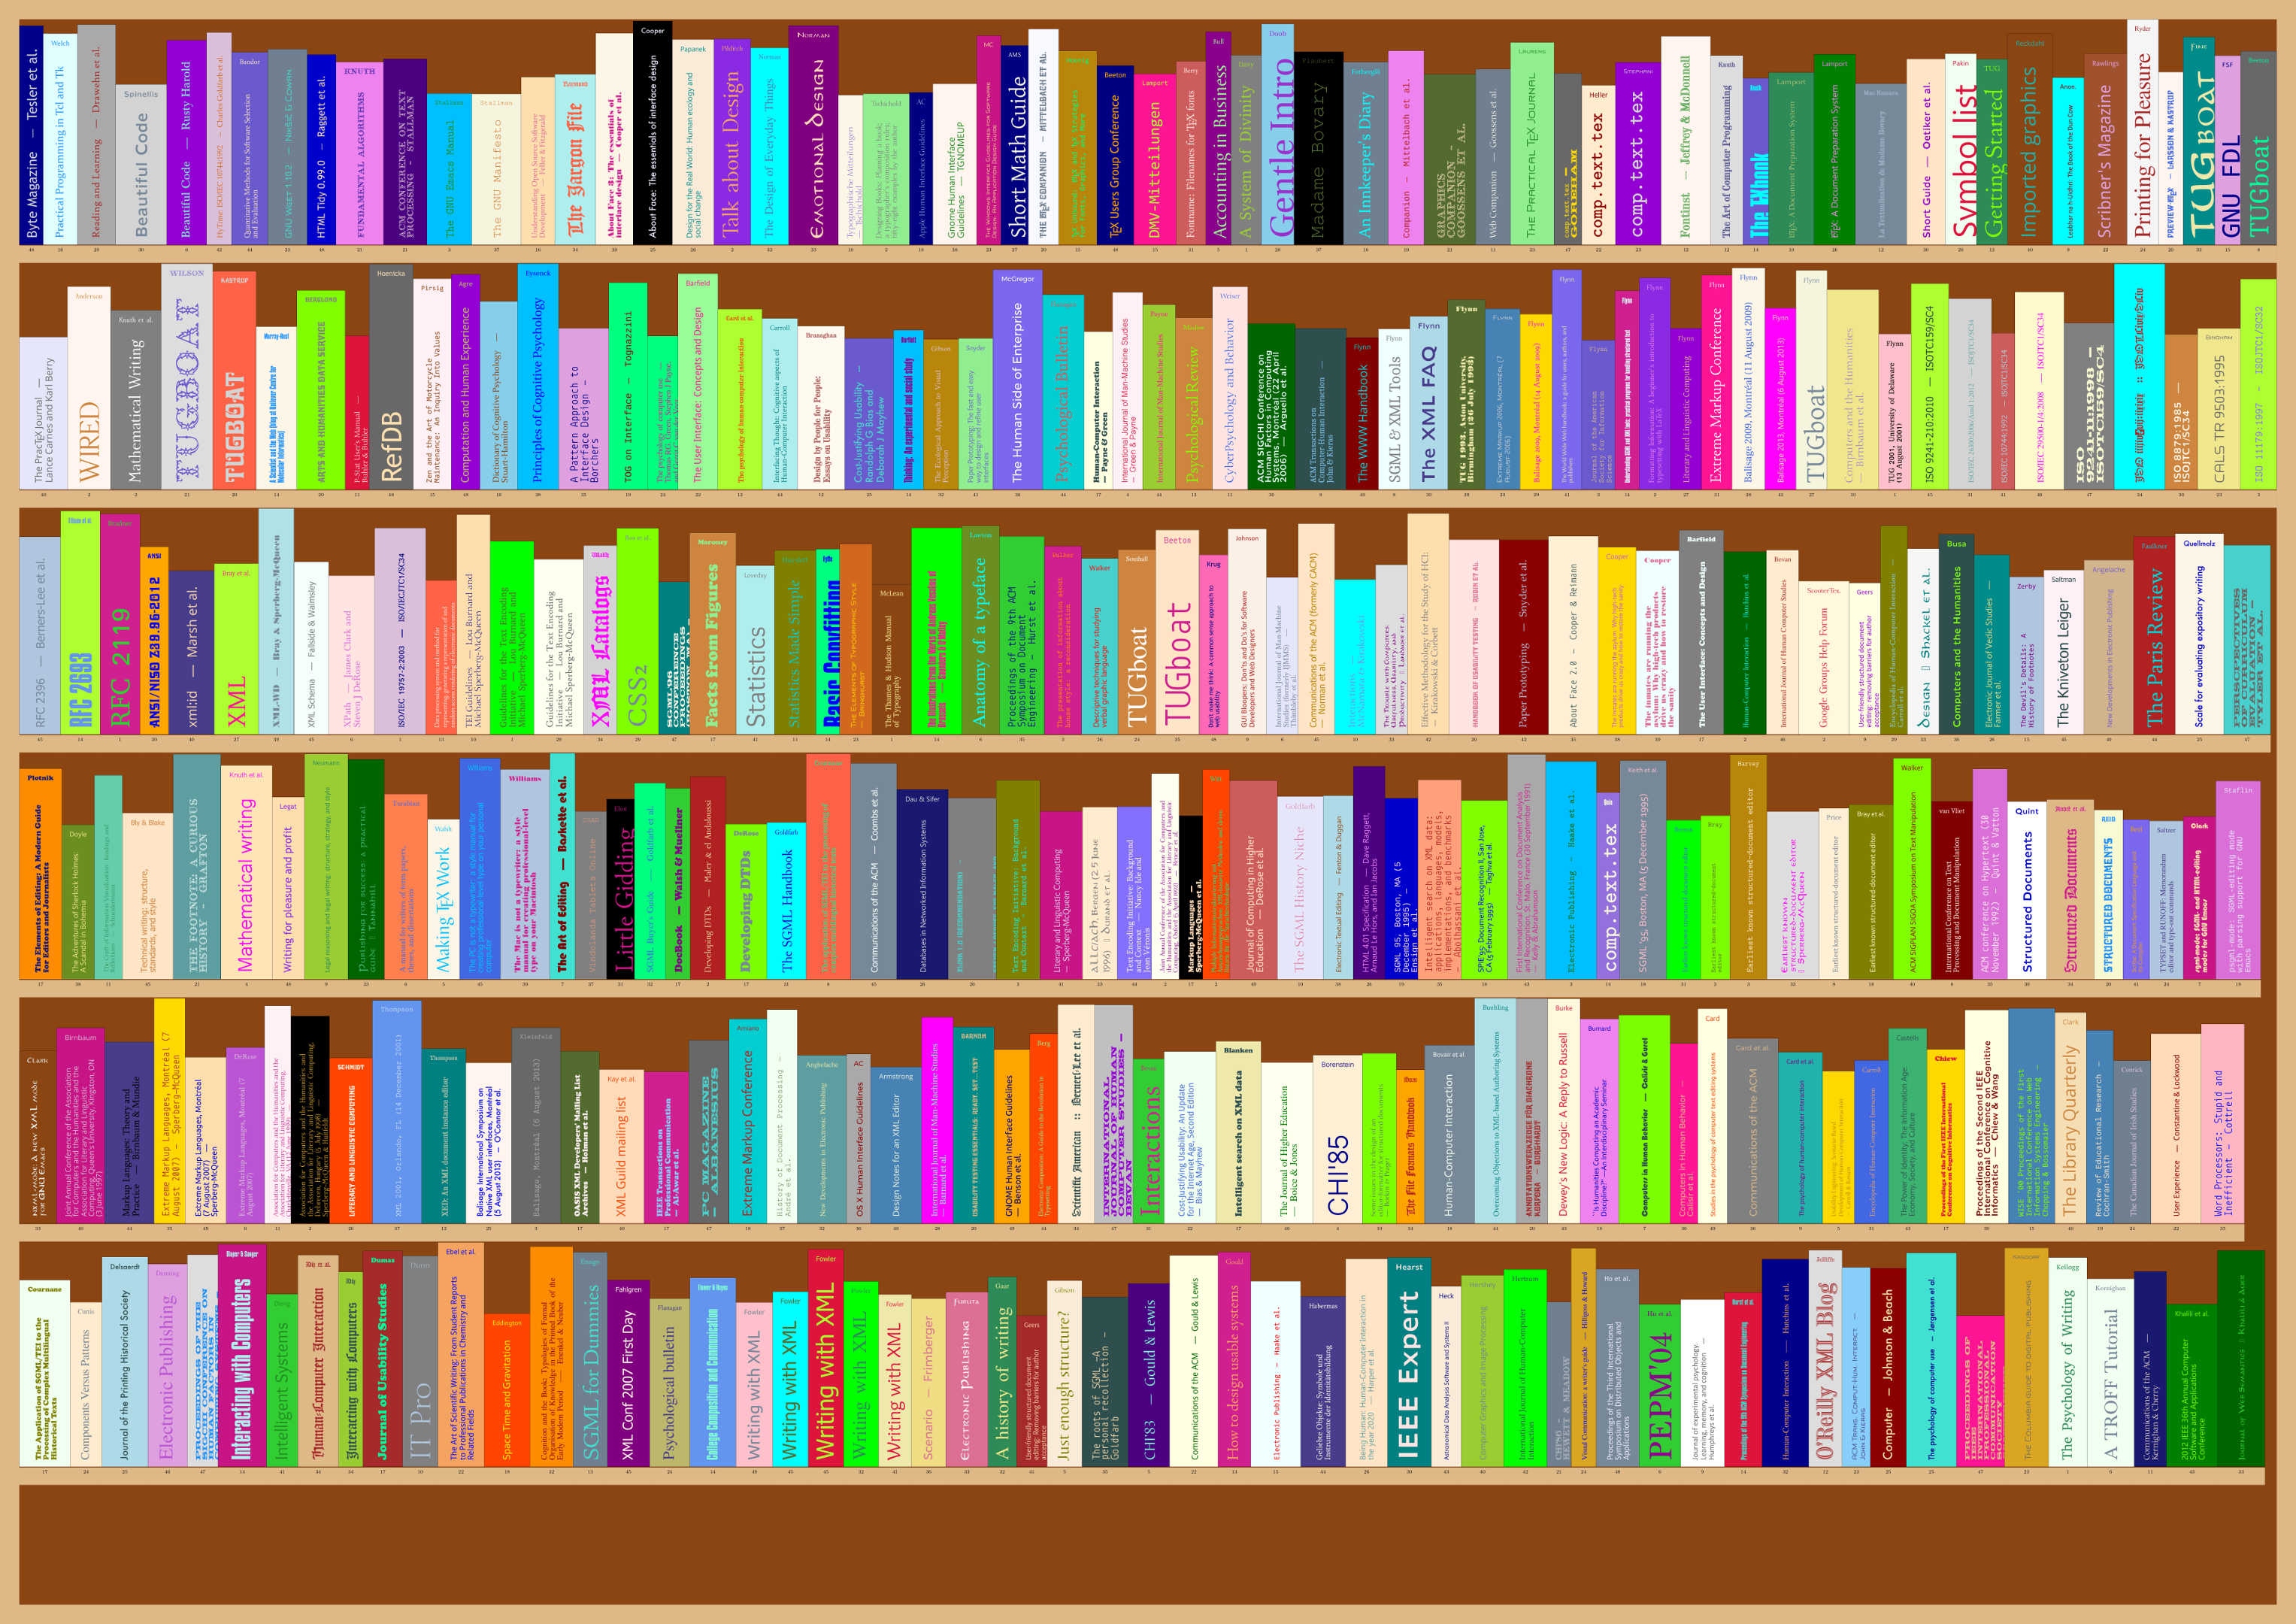
\includegraphics[width=.666\columnwidth]{myshelf.jpg}
% \end{abstract}
% \clearpage
% \tableofcontents
% \subsection*{Note on required and optional features}
% In this document, the keywords
%     {\sffamily {\smaller MUST}}, {\sffamily {\smaller MUST NOT}}, {\sffamily {\smaller REQUIRED}},
%     {\sffamily {\smaller SHALL}}, {\sffamily {\smaller SHALL NOT}}, {\sffamily {\smaller SHOULD}},
%     {\sffamily {\smaller SHOULD NOT}},
%     {\sffamily {\smaller RECOMMENDED}},
%     {\sffamily {\smaller MAY}}, and
%     {\sffamily {\smaller OPTIONAL}} have a specific
%     meaning when shown in {\sffamily {\smaller THIS TYPESTYLE}}, and
%     {\sffamily {\smaller MUST}} be interpreted as described in
%     RFC 2119 \parencite{rfc2119}.\par
% When shown in normal type, these words keep their conventional
%     contextual degree of meaning.\par
% \clearpage
% \section*{Latest changes}
% \subsection*{v.0.5 (2020-05-24)}
% \paragraph*{Finished initial testing}
% \begin{itemize}
% \item Replaced \textsf{hyperref}
% with \textsf{hypdoc} to avoid
% \emph{makeindex} bug\par
% \end{itemize}
% \subsection*{v.0.1 (2020-05-7)}
% \paragraph*{First packaged draft}
% \begin{itemize}
% \item Done manually from .tex file\par
% \end{itemize}
% \subsection*{v.0.4 (2020-05-19)}
% \paragraph*{Completed documentation}
% \begin{itemize}
% \item Updated note on bug in
% \emph{biber} when processing
% {\ttfamily{}sgml.bib}\par
% \item Removed {\ttfamily{}sgml.bib} as example
% until problems are resolved\par
% \item Backtracked on attempt to use the monographic
% title for articles, chapters, etc\par
% \item Revised notes on production\par
% \end{itemize}
% \subsection*{v.0.3 (2020-05-14)}
% \paragraph*{Finished first pass on documentation}
% \begin{itemize}
% \item Done preliminary testing\par
% \item Script adapted for Mac OS X\par
% \end{itemize}
% See p.\thinspace\pageref{changehistory} for earlier changes.
% \subsection*{Acknowledgments}
% Thanks to many people for the original
% suggestion; and to Isabel Yorke, Bethan Tovey-Walsh,
% Nelson Beebe, The \LaTeX{} Ninja, Stephan Lukasczyk,
% and others for their thesis bibliographies and
% testing comments.\par
% \clearpage
% \section{Documentation}
% During the era of the
% {\smaller COVID-19} lockdown, the popularity
% of group video messaging grew rapidly, both for
% business and domestic use. As people sought for what
% they believed to be more representative backgrounds
% than a messy kitchen, an untidy workroom, or a
% sterile blank wall, a well-populated bookshelf was a
% frequent choice.\par
% This package is for those who cannot use (or
% don't have, or don't want to use) such a bookshelf,
% but can still lay their hands on a bibliography or
% reference list in \BibTeX{} format — perhaps from a
% recent or long-forgotten thesis, book, article, or
% other document.\par
% \par\begingroup
%   \fboxsep1em\centering
%   \fbox{\begin{minipage}{0.8\columnwidth}\sffamily
%  \raggedright\parindent0pt
%  \parskip=.5\baselineskip
% \subsubsection*{\sffamily \XeLaTeX{} and \textsf{biblatex} and
%   \emph{biber}}
% To avoid problems with accented and other
%   characters, and to make it easier to maintain,
%   this document class uses only \XeLaTeX{} and
%   \textsf{biblatex} and
%   \emph{biber}.\par
% It will not work with the
%   \emph{pdflatex} or
%   \emph{bibtex} programs, and it does not
%   use the {\ttfamily{}.bst} files of old
%   \BibTeX{}.\par
% \end{minipage}}\par\endgroup
% This is a work-in-progress: there are bugs (see \vref{bugs}).\par
% \subsection{What the package does}
% The \textsf{bookshelf} package
%   generates what looks like shelves of book spines
%   from your list of references, using random
%   dimensions (within specified limits) in random but
%   contrasting colors, with a randomly-selected
%   typeface.\par
% It does this by creating a box (rectangle) for each
%   entry in your list, assigning colors to the background and
%   foreground, deciding on the layout and font, and then
%   stacking the boxes side-by-side as if they were letters on a
%   line.\par
% \subsection{Preparation}
% To get things ready for this, you need to install this
%   document class, and provide the following files.\par
% \begin{enumerate}
% \item Your \BibTeX{} file;
% \item A list of all the entry values;
% \item A list of all your usable text fonts;
% \item A command defining how many such fonts;
% \item A list of all the colors to choose from.
% \end{enumerate}
% These are explained in more detail in the subsections
%   below.\par
% All but the first of these can be generated by the
%   supplied shell script {\ttfamily{}prepdata.sh}. This
%   works on UNIX/GNU Linux and on Apple Mac OS X, and may work
%   in CygWin, but needs more work for plain Windows.\par
% \subsubsection{Your \BibTeX{} file}
% Your \BibTeX{} ({\ttfamily{}.bib}) file,
%     suitable for use with \emph{biber}
%     rather than \emph{bibtex}.\par
% Old \BibTeX{} files will work, but possibly not
%     optimally: if you want to update them, see \vref{bibchanges} for what to edit; but this is not
%     needed for this class.\par
% One thing that may help is to replace all the
%     old-style symbolic notation accented characters like
%     \verb|{\"a}| for
%     `ä' and
%     \verb|{\l}| for
%     `ł'. Not only is the symbolic
%     notation no longer needed because \XeLaTeX{} and the
%     \emph{biber} program handle
%     {\smaller UTF-8} characters, which the old
%     \emph{bibtex} program doesn't; the
%     discipline of replacing helps to reduce the problem of
%     unmatched curly braces, which is one of the biggest
%     sources of errors in \BibTeX{} files.\par
% If you have a bibliography in
%     \emph{EndNote},
%     \emph{Mendeley},
%     \emph{Zotero},
%     \emph{ProCite},
%     \emph{Reference Manager},
%     etc, you should be able to export it in either
%     \BibTeX{} or {\smaller RIS} format. A
%     {\smaller RIS} file can easily be
%     converted to \BibTeX{} by opening it in
%     \emph{JabRef} and saving it
%     as \BibTeX{}.\par
% \subsubsection{Entry values}
% A list of all the entry values from your \BibTeX{} file
%     (the unique names immediately after the document type),
%     each given as the argument to a
%     \verb|\makebook}{...}| command in a file called
%     {\ttfamily{}entries.tex}.\par
% \subsubsection{Font file list}\label{fontfiles}
% A set of 1–line files in a subdirectory called
%     {\ttfamily{}fontsel} representing of all the
%     usable text fonts on your system that you wish to use;
%     that is, excluding broken or partial fonts, symbols, math,
%     non-Latin characters or alphabets, and display or non-text
%     fonts.\par
% Each file {\sffamily {\smaller MUST}} be
%     numbered sequentially in its name (eg
%     {\ttfamily{}1.tex}, {\ttfamily{}2.tex},
%     {\ttfamily{}3.tex}, etc) and
%     {\sffamily {\smaller MUST}} contain a
%     \verb|\newfontface{SILmfont}{...}| command for
%     the font name \emph{and} a definition of its
%     name in a \verb|\SILmfontname{...}| command
%     (see the examples generated by the
%     {\ttfamily{}prepdata.sh} script). Be aware that
%     many fonts on your system may not be suitable for setting
%     normal text: see the comments in the script\par
% These files are entirely dependent on your system
%     because everyone has a different set of fonts.\par
% \subsubsection{Maximum number of fonts}
% A file called {\ttfamily{}pickfont.tex}
%     containing a
%     \verb|\setcounter{SIL@maxfont}{...}| command to
%     set the total number of the fonts which are represented in
%     the {\ttfamily{}fontsel} subdirectory above\par
% \subsubsection{List of colors}
% A list of all the colors represented by the
%     {\smaller SVG} palette used by the
%     \textsf{xcolor} package: the file created by
%     the script is called {\ttfamily{}svgnam.tex}.
%     This contains three definitions:\par
% \begin{enumerate}
% \item the command {\ttfamily{}\textbackslash{}SIL@svgcolname}
% which uses an {\ttfamily{}\textbackslash{}ifcase} command to
% return the name of the \emph{n}th color
% in alphabetical order;\par
% \item the command {\ttfamily{}\textbackslash{}SIL@svgcolval} which
% does the same to return the brightness value of that
% color, computed by the formula on \vpageref{bright} (see script for
% details);\par
% \item the counter {\ttfamily{}SIL@maxcolno} which holds
% the number of colors available.\par
% \end{enumerate}
% \subsection{Producing your bookshelf}
% This class comes with a file
%   {\ttfamily{}test.tex} which you can use to test your
%   file of references. It is initially set just to make the
%   {\ttfamily{}test.aux} file that
%   \emph{biber} needs to create your
%   {\ttfamily{}test.bbl} bibliography file; that is, it
%   will \emph{not} try to run the shell script
%   \emph{or} to create a bookshelf the first time
%   round, until everything else is ready.\par
% \begin{enumerate}
% \item Run the shell script with your
%       {\ttfamily{}.bib} filename as the argument,
%       eg;
% \iffalse
%<*ignore>
% \fi
\begin{lstlisting}[language={[LaTeX]TeX}]
$ ./prepdata.sh mythesis.bib
\end{lstlisting}
% \iffalse
%</ignore>
% \fi
% \item Edit the {\ttfamily{}test.tex} file and
%       change the name of the {\ttfamily{}.bib} file in
%       the {\ttfamily{}\textbackslash{}addbibresource} command to the
%       name of your own file\par 
% Leave the two lines {\ttfamily{}\textbackslash{}immediate} and
%       {\ttfamily{}\textbackslash{}input} commented out for the
%       moment;
% \item Delete any {\ttfamily{}test.aux} or
%       {\ttfamily{}test.bbl} files in the directory in
%       which you are doing this;
% \item Typeset the test file with \XeLaTeX{}. You should get
%     three messages:\par
% \iffalse
%<*ignore>
% \fi
\begin{lstlisting}[language={[LaTeX]TeX}]
LaTeX Warning: Empty bibliography on input line 12.
LaTeX Warning: There were undefined references.
Package biblatex Warning: Please (re)run Biber on the file:
(biblatex)                test
(biblatex)                and rerun LaTeX afterwards.
\end{lstlisting}
% \iffalse
%</ignore>
% \fi
% \item Process the test file with
%       \emph{biber}
%       (\emph{not} \emph{bibtex}). You will probably
%       get many warning messages: ignore them. If you get a
%       fatal error, however, you will need to find the problem
%       in your {\ttfamily{}.bib} file and fix it before
%       going any further.\par
% See also the known bug at item~\ref{sgmlbib} in the list on p.\thinspace\pageref{sgmlbib};
% \item Edit the test file and
%       \emph{un}comment the line starting
%       {\ttfamily{}\textbackslash{}input}, save the file, and retypeset
%       it twice.
% \end{enumerate}
% You should now have a {\smaller PDF} bookshelf!
%   The books are in the order in which they appear in your
%   {\ttfamily{}.bib} file because the script creates
%   the list of entries to process in that order, regardless of
%   what \emph{biblatex} or
%   \emph{biber} are configured to
%   do.\par
% \subsubsection{Options}
% The class comes set for making an
%     \textbf{\texttt{a0paper}} page (1189 mm × 841 mm
%     or 4′ 11″ × 2′ 10″) in
%     \textbf{\texttt{landscape}} mode, suitable for
%     large bibliographies. If you have a smaller
%     {\ttfamily{}.bib} file, or if you want
%     fewer volumes per page, you can change the paper
%     size option in the
%     {\ttfamily{}\textbackslash{}documentclass} command to a
%     smaller one: all the `A'
%     sizes from 5 to 0 are supported, plus the common
%     US office sizes including Ledger (Tabloid).\par
% There is also a \textbf{\texttt{portrait}} option to
%     produce the page in that format instead of
%     landscape.\par
%
% \subsection{Changes between \BibTeX{} fields and
%   \emph{biblatex}}\label{bibchanges}
% This has been expanded from the description provided in
%   \href{http://mirrors.ctan.org/macros/latex/contrib/biblatex/doc/biblatex.pdf\#page=33}{§2.3
%     of the online documentation for
%     \textsf{biblatex}} v3.14 (1 December
%   2019).\par
% This is for information only. You do not need to do any
%   of this to use the \index{bookshelf=\textsf{bookshelf} (class)}\textsf{bookshelf} document
%   class unless you encounter errors processing your
%   {\ttfamily{}.bib} file.\par
% \begin{enumerate}
% \item The entry type {\ttfamily{}@inbook}
%       (basically only use this where each chapter of the book
%       is written by a different author). See \href{http://mirrors.ctan.org/macros/latex/contrib/biblatex/doc/biblatex.pdf\#page=8}{§2.1.1} 
%       and \href{http://mirrors.ctan.org/macros/latex/contrib/biblatex/doc/biblatex.pdf\#page=33}{§2.3.1} 
%       for details.\par
% \item Replace {\ttfamily{}school} with {\ttfamily{}institution} for theses;
%       replace {\ttfamily{}publisher} with {\ttfamily{}organization} for manuals
% and conference sponsors;
%       and replace {\ttfamily{}address} with {\ttfamily{}location}. See \href{http://mirrors.ctan.org/macros/latex/contrib/biblatex/doc/biblatex.pdf\#page=17}{§2.2.2}, 
%       \href{http://mirrors.ctan.org/macros/latex/contrib/biblatex/doc/biblatex.pdf\#page=32}{§2.2.5}, 
%       and \href{http://mirrors.ctan.org/macros/latex/contrib/biblatex/doc/biblatex.pdf\#page=34}{§2.3.4} 
%       for details.\par
% \item The handling of certain types of titles. See \href{http://mirrors.ctan.org/macros/latex/contrib/biblatex/doc/biblatex.pdf\#page=35}{§2.3.5} 
%       for details. Replace {\ttfamily{}journal} with
%       {\ttfamily{}journaltitle} in {\ttfamily{}@article} entries.\par
% \item The field {\ttfamily{}series}: only
%       use it for journal series; for the main title of
%       multi-volume works use {\ttfamily{}maintitle}.
%       See \href{http://mirrors.ctan.org/macros/latex/contrib/biblatex/doc/biblatex.pdf\#page=17}{§2.2.2} 
%       and \href{http://mirrors.ctan.org/macros/latex/contrib/biblatex/doc/biblatex.pdf\#page=37}{§2.3.7} 
%       for details.\par
% \item The fields {\ttfamily{}year} and {\ttfamily{}month} must be
%       integers; {\ttfamily{}month} {\sffamily {\smaller MUST NOT}} be
%       alphabetic. The field {\ttfamily{}date} {\sffamily {\smaller MUST}} be an
%       {\smaller ISO} 8601 date in the format
%       {\ttfamily{}yyyy-mm-dd}. See \href{http://mirrors.ctan.org/macros/latex/contrib/biblatex/doc/biblatex.pdf\#page=17}{§2.2.2}, 
%       \href{http://mirrors.ctan.org/macros/latex/contrib/biblatex/doc/biblatex.pdf\#page=38}{§2.3.8}, 
%       and \href{http://mirrors.ctan.org/macros/latex/contrib/biblatex/doc/biblatex.pdf\#page=39}{§2.3.9} 
%       for details.\par
% \item The field {\ttfamily{}edition} must
%       be an integer with no ordinal indicator or abbreviation
%       `ed'. See \href{http://mirrors.ctan.org/macros/latex/contrib/biblatex/doc/biblatex.pdf\#page=17}{§2.2.2} 
%       for details.\par
% \item Replace {\ttfamily{}key} with
%       {\ttfamily{}label}. See \href{http://mirrors.ctan.org/macros/latex/contrib/biblatex/doc/biblatex.pdf\#page=33}{§2.3.2} 
%       for details.\par
% \end{enumerate}
% Most of this is for creating new entries. For converting
%   \BibTeX{} files for use with
%   \emph{biblatex}, just change the field
%   names as in items 2, 3, 4, and 7; and make sure your months
%   and editions are integers.\par
% \subsection{Bugs}\label{bugs}
% Some things don't yet work as they should, and
%   there are some features that may or may not make
%   the final cut.\par
% \begin{enumerate}
% \item The shell script doesn't run on Windows
%       because I don't have any Windows. If someone
%       would write some Powershell I could include it
%       in a later version.\par
% \item There is no conscious
%       `line'-breaking when a
%       row of books comes to the
%       {\ttfamily{}\textbackslash{}pagewidth}, and as it is
%       deliberately set
%       {\ttfamily{}\textbackslash{}raggedright} (because you
%       can't hyphenate a book and variable space
%       between books seems to be a silly idea), there
%       is no filler at the ends of lines to complete
%       the `shelf' (which is
%       in any case just a bar below each
%       book).\par
% \item \label{sgmlbib}A test with a bibliography file from
%       Nelson Beebe's collection
%       ({\ttfamily{}sgml.bib}) generated a
%       {\ttfamily{}test.bbl} with a missing
%       closing curly brace, terminating (or rather,
%       failing to terminate) the
%       {\ttfamily{}\textbackslash{}name} command for an entry.
%       This appears to be a known bug in
%       \emph{biber} which is
%       being fixed in the version 2.15.\par
% \item There seems to be a recurrent problem with
%       certain entries and certain fonts where the
%       length of the title is measured as 0.0pt which
%       causes an unresolvable problem for the routine
%       which assigns space and layout. Any
%       suggestions as to why this occurs are
%       welcomed.\par
% \item The objective of the field re-expressions
%       (see \vref{fields}) was to make sure the book
%       spine for journal {\ttfamily{}@article}, {\ttfamily{}@incollection}, and
%       {\ttfamily{}@inbook} entry
%       types reflected the \emph{book}
%       or \emph{journal} title, not the
%       title of the article or chapter. This may or
%       may not be a good idea.\par
% \item During development, it became obvious that
%       the number of fonts on many systems can be
%       very large. The
%       {\ttfamily{}prepdata.sh} script
%       currently includes the exclusions I made on
%       {\smaller UNIX}/{\smaller GNU}
%       Linux and Apple Mac {\smaller OS X} in
%       order to get a set of fonts that did not issue
%       errors (bearing in mind we are using
%       \textsf{fontspec}, so for simplicity
%       the script deals only with TrueType and
%       OpenType fonts, not Postscript Type 1 or
%       Type 3, or font packaging systems like
%       \emph{Suitcase} or True
%       Type Collections). I am not aware of any
%       easily-accessible machine-readable list or
%       {\smaller API} for identifying normal
%       text fonts by name (there are commercial
%       databases but that is outside the scope of
%       this document class).\par
% \end{enumerate}
% \StopEventually{\label{endcode}%
%   \clearpage
%   \newgeometry{left=3cm}%
%   \addcontentsline{toc}{section}{Change History}%
%   \label{changehistory}%
%   \PrintChanges
%   \clearpage
%   \label{codeindex}%
%   \addcontentsline{toc}{section}{Index}%
%   \PrintIndex}
% \addtolength{\CPKrevmarg}{\widthof{\LabelFont{AddToShipoutPictureBG}}}
% \newgeometry{left=\CPKrevmarg}
% \message{Margin reset to \the\CPKrevmarg, to fit <AddToShipoutPictureBG>}
% \iffalse
%<*class>
% \fi
% \clearpage
% \section{Implementation}\label{setup}
% \par
% \subsection{Auto-initialisation}\label{setup:autoinit}
% This section is added automatically by \textit{ClassPack} 
% as a preamble to all classes and style packages. 
% The \textsf{fixltx2e} package, which used to be included
% automatically, is no longer preloaded, as its
% features are now a part of the latest \LaTeXe\ kernel.\par
% The code starts with identity and requirements which are 
% generated automatically as needed by the Doc\TeX\ system.
% For details see the \textsf{ltxdoc} package documentation.
% \par\smallskip
% \begingroup\color{DarkRed}\footnotesize
% \leavevmode\enspace{\scriptsize1}\quad{\ttfamily\textbackslash NeedsTeXFormat\{LaTeX2e\}[2017/04/15]}\\
% \leavevmode\enspace{\scriptsize2}\quad{\ttfamily\textbackslash ProvidesClass\{bookshelf\}[2020/05/24 v0.5}\\
% \leavevmode\enspace{\scriptsize3}\qquad{\ttfamily Turn your bibliography into a bookshelf image]}\\\endgroup
% \setcounter{CodelineNo}{3}
% \begin{CPK@package}{fix-cm}
% Preloaded functions to override the default \LaTeX\
% step-size font sizes (which can still be used,
% but are no longer restrictions).\par
%    \begin{macrocode}
\RequirePackage{fix-cm}
%    \end{macrocode}
% \end{CPK@package}
% \begin{CPK@option}{svgnames}
% Pass the \textbf{\texttt{svgnames}} option to the
% \textsf{xcolor} package if that gets loaded later.
% This avoids a conflict with any other packages
% (eg \textsf{hyperref}) which use their own default
% is when they load \textsf{xcolor}.\par
%    \begin{macrocode}
  \PassOptionsToPackage{svgnames}{xcolor}
%    \end{macrocode}
% \end{CPK@option}
% \subsection{Options}\label{options}
% \iffalse
%% 
%% ****************************************************************** 
%% 
%% Options
% \fi
% The paper size and orientation are the only two valid
%   options, both of which are the same as the standard
%   documentclass options, and will be passed to the underlying
%   class automatically, but they need recording so that they
%   can be used by the \textsf{geometry}
%   package. The default is for A0 paper, landscape.\par
%    \begin{macrocode}
\def\SIL@paper{a0paper}%
\DeclareOption{a0paper}{%
    \def\SIL@paper{a0paper}%
    \setlength\paperheight {1189mm}%
    \setlength\paperwidth  {841mm}}
\DeclareOption{a1paper}{%
    \def\SIL@paper{a1paper}%
    \setlength\paperheight {841mm}%
    \setlength\paperwidth  {594mm}}
\DeclareOption{a2paper}{%
    \def\SIL@paper{a2paper}%
    \setlength\paperheight {594mm}%
    \setlength\paperwidth  {420mm}}
\DeclareOption{a3paper}{%
    \def\SIL@paper{a3paper}%
    \setlength\paperheight {420mm}%
    \setlength\paperwidth  {297mm}}
\DeclareOption{a4paper}{%
    \def\SIL@paper{a4paper}%
    \setlength\paperheight {297mm}%
    \setlength\paperwidth  {210mm}}
\DeclareOption{a5paper}{%
    \def\SIL@paper{a5paper}%
    \setlength\paperheight {210mm}%
    \setlength\paperwidth  {148mm}}
\DeclareOption{b5paper}{%
    \def\SIL@paper{b5paper}%
    \setlength\paperheight {250mm}%
    \setlength\paperwidth  {176mm}}
\DeclareOption{letterpaper}{%
    \def\SIL@paper{letterpaper}%
    \setlength\paperheight {11in}%
    \setlength\paperwidth  {8.5in}}
\DeclareOption{legalpaper}{%
    \def\SIL@paper{legalpaper}%
    \setlength\paperheight {14in}%
    \setlength\paperwidth  {8.5in}}
\DeclareOption{executivepaper}{%
    \def\SIL@paper{executivepaper}%
    \setlength\paperheight {10.5in}%
    \setlength\paperwidth  {7.25in}}
\DeclareOption{ledgerpaper}{%
    \def\SIL@paper{ledgerpaper}%
    \setlength\paperheight {17in}%
    \setlength\paperwidth  {11in}}
\DeclareOption{tabloidpaper}{%
    \def\SIL@paper{tabloidpaper}%
    \setlength\paperheight {17in}%
    \setlength\paperwidth  {11in}}
\def\SIL@orient{landscape}%
\DeclareOption{landscape}{%
    \def\SIL@orient{landscape}%
    \setlength\@tempdima   {\paperheight}%
    \setlength\paperheight {\paperwidth}%
    \setlength\paperwidth  {\@tempdima}}
\DeclareOption{portrait}{%
    \def\SIL@orient{}}
%    \end{macrocode}
% \subsection{Load the document base class}\label{classload}
% \iffalse
%% 
%% ****************************************************************** 
%% 
%% Load the document base class
% \fi
% This class is based on the standard \LaTeX{}
%   \DescribeClass{report}\textsf{report} class, with no special options
%   except the extra sizes defined above. The default is A0
%   paper, landscape.\par
%    \begin{macrocode}
\DeclareOption*{\ClassWarning{bookshelf}{%
    Unknown option `\CurrentOption', please RTFM}}
\ProcessOptions\relax
\LoadClass{report}
%    \end{macrocode}
%\iffalse
%%
%% Packages required for the class or package
%% 
% \fi
% \subsection{Packages required for the class or
%     package}\label{clspackages}
% \begin{CPK@package}{fontspec}
% Font specification setup for use with \XeLaTeX{}.
% \iffalse
%% Font specification setup for use with \XeLaTeX{}.
% \fi
%    \begin{macrocode}
\RequirePackage{fontspec}%
%    \end{macrocode}
% \end{CPK@package}
% \begin{CPK@package}{calc}
% Required for calculations involving lengths or counters,
% such as changes to widths for margin adjustment.
% \iffalse
%% Required for calculations involving lengths or counters, such as changes to widths for margin adjustment.
% \fi
%    \begin{macrocode}
\RequirePackage{calc}%
%    \end{macrocode}
% \end{CPK@package}
% \begin{CPK@package}{fp}
% Used for fixed-point calculations;
% \iffalse
%% Used for fixed-point calculations
% \fi
%    \begin{macrocode}
\RequirePackage{fp}%
%    \end{macrocode}
% \end{CPK@package}
% \begin{CPK@package}{graphicx}
% Provide for graphics (PNG, JPG, or PDF format (only) for
% pdflatex; EPS format (only) for standard \LaTeX{}).
% \iffalse
%% Provide for graphics (PNG, JPG, or PDF format (only) for pdflatex; EPS format (only) for standard \LaTeX{}).
% \fi
%    \begin{macrocode}
\RequirePackage{graphicx}%
%    \end{macrocode}
% \end{CPK@package}
% \begin{CPK@package}{xcolor}
% Provide color.
% \iffalse
%% Provide color.
% \fi
%    \begin{macrocode}
\RequirePackage{xcolor}%
  \@ifundefined{T}{%
	    \newcommand{\T}[2]{{\fontencoding{T1}%
	      \selectfont#2}}}{}
%    \end{macrocode}
% There seems to be a bug in the T1 encoding of some package
% (unidentified, but possibly \textsf{xcolor}) which
% uses the command {\ttfamily{}\textbackslash{}T1}, which is an
% impossibility (no digits allowed in command names). So we fake
% it here to stop \LaTeX{} complaining, by dropping the first
% argument on the floor.
% \end{CPK@package}
% \begin{CPK@package}{eso-pic}
% Add picture commands (or backgrounds) to every page.
% \iffalse
%% Add picture commands (or backgrounds) to every page.
% \fi
%    \begin{macrocode}
\RequirePackage{eso-pic}%
%    \end{macrocode}
% \end{CPK@package}
% \begin{CPK@package}{geometry}
% Package for establishing margins and text area.
% \iffalse
%% Package for establishing margins and text area.
% \fi
%    \begin{macrocode}
\RequirePackage[\SIL@paper,\SIL@orient,nohead,
  nofoot,margin=1cm]{geometry}%
%    \end{macrocode}
% \end{CPK@package}
% \begin{CPK@package}{biblatex}
% Use \textsf{biblatex} instead of \BibTeX{};
% \iffalse
%% Use biblatex instead of \BibTeX{}
% \fi
%    \begin{macrocode}
\RequirePackage[backend=biber,style=authoryear,
  doi=true,isbn=true,url=true,uniquename=false]{biblatex}%
  \AtBeginDocument{%
	    \setlength{\bibitemsep}{1ex}%
	    \setlength{\bibnamesep}{1.5\itemsep}%
	    \defbibheading{shortbib}[References]%
	      {\section{#1}}}
	  \@ifpackagewith{babel}{british}{%
	    \DeclareLanguageMapping{british}%
	      {british-apa}}{\relax}
  \providetoggle{blx@skipbiblist}
%    \end{macrocode}
% \end{CPK@package}
% 
% \subsection{Non-package resources}
% \iffalse
%% 
%% ****************************************************************** 
%% 
%% Non-package resources
% \fi
% \begin{CPK@file}{random.tex}\label{file--random.tex}
% There is one resource not available in packaged form,
%     the module that lets \LaTeX{} create random values. This is
%     in {\ttfamily{}random.tex}, which on the author's
%     system is hiding in a directory
%     {\ttfamily{}texmf/tex/generic/genmisc/}, in the
%     {\ttfamily{}texmf-dist} tree, and indexed by an
%     {\ttfamily{}ls-R} database, so it should therefore
%     be findable by any \TeX{} system.\par
%    \begin{macrocode}
\input{random.tex}
%    \end{macrocode}
% \end{CPK@file}
% \subsection{The code}
% \iffalse
%% 
%% ****************************************************************** 
%% 
%% The code
% \fi
% This is beta software: the code is messy and covered in
%   tracing output.\par
% \subsubsection{Font selection}\label{fonts}
% \begin{CPK@counter}{maxfont}\label{counter--maxfont}
% This is set in the {\ttfamily{}\textbackslash{}input} file
%       {\ttfamily{}pickfont.tex}, which is created by
%       the preparatory data script
%       {\ttfamily{}prepdata.sh}. It is the number of
%       working text fonts found on the system.\par
%    \begin{macrocode}
\newcounter{SIL@maxfont}
%    \end{macrocode}
% \end{CPK@counter}
% \begin{CPK@counter}{SIL@fontsel}\label{counter--SIL@fontsel}
% This is set to a random number between one and
%       \DescribeCounter{SIL@maxfont}{\ttfamily{}SIL@maxfont}, and used as the
%       name of the file containing the font name.\par
%    \begin{macrocode}
\newcounter{SIL@fontsel}
%    \end{macrocode}
% \end{CPK@counter}
% \begin{CPK@file}{pickfont.tex}\label{file--pickfont.tex}
% This file is created by the preparatory data script
%       {\ttfamily{}prepdata.sh} after it sets up the
%       subdirectory list of valid text fonts. It sets the value
%       of \DescribeCounter{SIL@maxfont}{\ttfamily{}SIL@maxfont}.\par
%    \begin{macrocode}
\input{pickfont.tex}
%    \end{macrocode}
% \end{CPK@file}
% \subsubsection{Color selection}\label{color}
% \begin{CPK@counter}{SIL@maxcolno}\label{counter--SIL@maxcolno}
% This value is set at the end of the file
%       {\ttfamily{}svgnam.tex}. This is the number of
%       color names found by the routine in
%       {\ttfamily{}prepdata.sh} which extracts the color
%       names.\par
%    \begin{macrocode}
\newcounter{SIL@maxcolno}
%    \end{macrocode}
% \end{CPK@counter}
% \begin{CPK@file}{svgnam.tex}\label{file--svgnam.tex}
% The preparatory data script
%       {\ttfamily{}prepdata.sh} retrieves the colors named
%       in the \textbf{\texttt{svgnames}} option to the
%       \textsf{xcolor} package and instantiates them
%       as a \LaTeX{} {\ttfamily{}\textbackslash{}ifcase} list in the file
%       {\ttfamily{}svgnam.tex} as the command
%       {\ttfamily{}\textbackslash{}SIL@svgcolname}.\par
%    \begin{macrocode}
\newcommand{\SIL@svgcolname}[1]{\ifcase#1 
AliceBlue\or
AntiqueWhite\or
Aqua\or
Aquamarine\or
Azure\or
Beige\or
Bisque\or
Black\or
BlanchedAlmond\or
Blue\or
BlueViolet\or
Brown\or
BurlyWood\or
CadetBlue\or
Chartreuse\or
Chocolate\or
Coral\or
CornflowerBlue\or
Cornsilk\or
Crimson\or
Cyan\or
DarkBlue\or
DarkCyan\or
DarkGoldenrod\or
DarkGray\or
DarkGreen\or
DarkGrey\or
DarkKhaki\or
DarkMagenta\or
DarkOliveGreen\or
DarkOrange\or
DarkOrchid\or
DarkRed\or
DarkSalmon\or
DarkSeaGreen\or
DarkSlateBlue\or
DarkSlateGray\or
DarkSlateGrey\or
DarkTurquoise\or
DarkViolet\or
DeepPink\or
DeepSkyBlue\or
DimGray\or
DimGrey\or
DodgerBlue\or
FireBrick\or
FloralWhite\or
ForestGreen\or
Fuchsia\or
Gainsboro\or
GhostWhite\or
Gold\or
Goldenrod\or
Gray\or
Green\or
GreenYellow\or
Grey\or
Honeydew\or
HotPink\or
IndianRed\or
Indigo\or
Ivory\or
Khaki\or
Lavender\or
LavenderBlush\or
LawnGreen\or
LemonChiffon\or
LightBlue\or
LightCoral\or
LightCyan\or
LightGoldenrod\or
LightGoldenrodYellow\or
LightGray\or
LightGreen\or
LightGrey\or
LightPink\or
LightSalmon\or
LightSeaGreen\or
LightSkyBlue\or
LightSlateBlue\or
LightSlateGray\or
LightSlateGrey\or
LightSteelBlue\or
LightYellow\or
Lime\or
LimeGreen\or
Linen\or
Magenta\or
Maroon\or
MediumAquamarine\or
MediumBlue\or
MediumOrchid\or
MediumPurple\or
MediumSeaGreen\or
MediumSlateBlue\or
MediumSpringGreen\or
MediumTurquoise\or
MediumVioletRed\or
MidnightBlue\or
MintCream\or
MistyRose\or
Moccasin\or
NavajoWhite\or
Navy\or
NavyBlue\or
OldLace\or
Olive\or
OliveDrab\or
Orange\or
OrangeRed\or
Orchid\or
PaleGoldenrod\or
PaleGreen\or
PaleTurquoise\or
PaleVioletRed\or
PapayaWhip\or
PeachPuff\or
Peru\or
Pink\or
Plum\or
PowderBlue\or
Purple\or
Red\or
RosyBrown\or
RoyalBlue\or
SaddleBrown\or
Salmon\or
SandyBrown\or
SeaGreen\or
Seashell\or
Sienna\or
Silver\or
SkyBlue\or
SlateBlue\or
SlateGray\or
SlateGrey\or
Snow\or
SpringGreen\or
SteelBlue\or
Tan\or
Teal\or
Thistle\or
Tomato\or
Turquoise\or
Violet\or
VioletRed\or
Wheat\or
White\or
WhiteSmoke\or
Yellow\or
YellowGreen\or
Black\fi}

\newcommand{\SIL@svgcolval}[1]{\ifcase#1 
0.96633\or
0.929923\or
0.871206\or
0.893092\or
0.985874\or
0.953778\or
0.913011\or
0\or
0.932641\or
0.260768\or
0.379297\or
0.349085\or
0.74815\or
0.570779\or
0.866469\or
0.529816\or
0.647294\or
0.576475\or
0.971909\or
0.433686\or
0.871206\or
0.142119\or
0.474807\or
0.561714\or
0.664\or
0.325856\or
0.664\or
0.705841\or
0.302953\or
0.388309\or
0.670841\or
0.396012\or
0.26755\or
0.675762\or
0.686451\or
0.281846\or
0.284935\or
0.284935\or
0.704877\or
0.35734\or
0.517671\or
0.675787\or
0.41\or
0.41\or
0.54021\or
0.361443\or
0.982202\or
0.458943\or
0.555878\or
0.864\or
0.97393\or
0.856285\or
0.683662\or
0.5\or
0.415632\or
0.897087\or
0.5\or
0.981852\or
0.625264\or
0.504136\or
0.19626\or
0.996035\or
0.890633\or
0.905664\or
0.956157\or
0.857112\or
0.973957\or
0.814506\or
0.634585\or
0.972435\or
0.864229\or
0.970187\or
0.828\or
0.835978\or
0.828\or
0.793828\or
0.727452\or
0.608906\or
0.764286\or
0.516182\or
0.522335\or
0.522335\or
0.758883\or
0.9923\or
0.831264\or
0.677159\or
0.947156\or
0.555878\or
0.245459\or
0.718037\or
0.209658\or
0.501212\or
0.513837\or
0.604404\or
0.480155\or
0.829725\or
0.726351\or
0.412174\or
0.148714\or
0.989148\or
0.920006\or
0.909698\or
0.891886\or
0.130384\or
0.130384\or
0.96388\or
0.482701\or
0.507329\or
0.728803\or
0.539791\or
0.598277\or
0.901054\or
0.883282\or
0.87941\or
0.578431\or
0.945407\or
0.88424\or
0.58891\or
0.821492\or
0.710864\or
0.839601\or
0.277939\or
0.490918\or
0.607101\or
0.430078\or
0.349771\or
0.646416\or
0.718648\or
0.470014\or
0.967932\or
0.40977\or
0.752\or
0.759198\or
0.413618\or
0.491035\or
0.491035\or
0.984857\or
0.841347\or
0.481407\or
0.726393\or
0.435603\or
0.781595\or
0.592817\or
0.771583\or
0.669428\or
0.43929\or
0.882294\or
1\or
0.96\or
0.965401\or
0.732944\or
0\fi}

\setcounter{SIL@maxcolno}{151}

%    \end{macrocode}
% \end{CPK@file}
% \begin{CPK@counter}{SIL@loopcount}\label{counter--SIL@loopcount}
% The random font selection is done in a loop because
%       of the need to test the values. This counter counts the
%       iterations…\par
%    \begin{macrocode}
\newcounter{SIL@loopcount}
%    \end{macrocode}
% \end{CPK@counter}
% \begin{CPK@counter}{SIL@maxloop}\label{counter--SIL@maxloop}
% …and this one the limit.\par
%    \begin{macrocode}
\newcounter{SIL@maxloop}
%    \end{macrocode}
% \end{CPK@counter}
% \begin{CPK@counter}{SIL@bgcolno}\label{counter--SIL@bgcolno}
% The colors are selected numerically. This value is
%       the background color of the spine of a book.\par
%    \begin{macrocode}
\newcounter{SIL@bgcolno}
%    \end{macrocode}
% \end{CPK@counter}
% \begin{CPK@counter}{SIL@fgcolno}\label{counter--SIL@fgcolno}
% And this is the foreground color, used to typeset
%       the title and author on the spine of a book.\par
%    \begin{macrocode}
\newcounter{SIL@fgcolno}
%    \end{macrocode}
% \end{CPK@counter}
% \begin{CPK@length}{\splitpoint}\label{length--splitpoint}
% To make sure that \DescribeCounter{SIL@bgcolno}{\ttfamily{}SIL@bgcolno} and \DescribeCounter{SIL@fgcolno}{\ttfamily{}SIL@fgcolno}
%       are distinct, we will need to pick one
%       `dark' and one
%       `light', crudely distinguished by
%       examining their `brightness'
%       (monochrome intensity value) using the formula
%       \label{bright}\(b=\sqrt(.241r^2+.691g^2+.068b^2)\) due to \href{https://www.nbdtech.com/Blog/archive/2008/04/27/Calculating-the-Perceived-Brightness-of-a-Color.aspx}{Nir 
% Dobovizki}. From inspection, the modal point of
%       the {\smaller SVG} values occurs around 0.6, so
%       use use this to determine if the randomly-selected color
%       is `dark' or
%       `light'. Because it's a decimal
%       fraction, we express it as a dimension and strip off the
%       `pt' later.\par
%    \begin{macrocode}
\newlength{\SIL@splitpoint}
\setlength{\SIL@splitpoint}{0.6pt}
%    \end{macrocode}
% \end{CPK@length}
% \begin{CPK@macro}{\SIL@bgcol}\label{macro--SIL@bgcol}
% We establish defaults for the background color…\par
%    \begin{macrocode}
\def\SIL@bgcol{White}
%    \end{macrocode}
% \end{CPK@macro}
% \begin{CPK@macro}{\SIL@fgcol}\label{macro--SIL@fgcol}
% …and the foreground color.\par
%    \begin{macrocode}
\def\SIL@fgcol{Black}
%    \end{macrocode}
% \end{CPK@macro}
% \begin{CPK@length}{\SIL@bgval}\label{length--SIL@bgval}
% The values computed by the
%       {\ttfamily{}prepdata.sh} script and stored in
%       {\ttfamily{}svgnam.tex} are decimal fractions,
%       to they need to be retrieved as lengths. This is the
%       background value…\par
%    \begin{macrocode}
\newlength{\SIL@bgval}
%    \end{macrocode}
% \end{CPK@length}
% \begin{CPK@length}{\SIL@fgval}\label{length--SIL@fgval}
% …and the foreground value.\par
%    \begin{macrocode}
\newlength{\SIL@fgval}
%    \end{macrocode}
% \end{CPK@length}
% \begin{CPK@length}{\SIL@bgfgdiff}\label{length--SIL@bgfgdiff}
% The `dark' or
%       `light' test discussed above also
%       needs to test if the values are too close to the
%       splitpoint. By examination, if the values have an
%       absolute difference of 0.2 they should be visually
%       distinct enough. The difference is calculated and stored
%       in this length variable, as it's a decimal fraction.\par
%    \begin{macrocode}
\newlength{\SIL@bgfgdiff}
%    \end{macrocode}
% \end{CPK@length}
% \begin{CPK@switch}{\SIL@notyetcols}\label{switch--SIL@notyetcols}
% In the testing for colors, the nested conditionals
%       set this switch true or false, so that it can be used to
%       control the iteration through successive attempts to find
%       suitable random values.\par
%    \begin{macrocode}
\newif\ifSIL@notyetcols
%    \end{macrocode}
% \end{CPK@switch}
% \subsubsection{Page border setup}\label{borders}
% \begin{CPK@macro}{\AddToShipoutPictureBG}\label{macro--AddToShipoutPictureBG}
% The page background color is set to a pale brown
%       roughly matching the pine veneer of IKEA bookcases, with
%       the inner page (behind the books) in a dark shadow
%       brown. The technique for imposing a colored margin is
%       due to \href{https://tex.stackexchange.com/questions/7725/how-to-set-a-certain-color-other-than-white-to-margin-areas}{Ulrike 
% Fischer} and uses the commands from the
%       \textsf{eso-pic} package.\par
%    \begin{macrocode}
\pagecolor{BurlyWood}
\AddToShipoutPictureBG{%
 \AtTextLowerLeft{\color{SaddleBrown}%
   \rule[-\footskip]{\textwidth}{%
     \dimexpr\textheight+\footskip}}}
%    \end{macrocode}
% \end{CPK@macro}
% \subsubsection{Size and shape}\label{sizeshape}
% Each book is assigned a random height and width,
%     within the bounds set by the maxima and minima. The final
%     dimensions may then be modified by the choice of layout
%     and font.\par
%    \begin{macrocode}
\newlength{\SIL@bookheight}
\newlength{\SIL@bookwidth}
\newlength{\SIL@minbookwidth}
\newlength{\SIL@maxbookwidth}
\newlength{\SIL@minbookheight}
\newlength{\SIL@maxbookheight}
%    \end{macrocode}
% \subsubsection{Title and author dimensions}\label{titling}
% The title and author need to be measured, and
%     decisions are made about what size they need to be. The
%     two layouts (author separately at the top, and author
%     inline to title) are distinguished with the
%     {\ttfamily{}\textbackslash{}SIL@topauthor} conditional. If the title
%     (with or without the author can fit on one line (rather
%     than multiple lines) this is signalled with the
%     {\ttfamily{}\textbackslash{}SIL@titleoneline} conditional.\par
%    \begin{macrocode}
\newlength{\SIL@titlewidth}
\newlength{\SIL@authorwidth}
\newlength{\SIL@titleheight}
\newlength{\SIL@authorheight}
\newlength{\SIL@scaledtitle}
\newlength{\SIL@heightfortitle}
\newbox\SIL@titlebox
\newif\ifSIL@topauthor
\newif\ifSIL@titleoneline
%    \end{macrocode}
% \subsubsection{Handling the math}
% \begin{CPK@counter}{SIL@scale}\label{counter--SIL@scale}
% To extract the integer part of a fixed-point value,
%       we define a simple strip which uses the integer and
%       throws away the rest. The integer ends up in this
%       counter.\par
%    \begin{macrocode}
\newcounter{SIL@scale}
%    \end{macrocode}
% \end{CPK@counter}
% \begin{CPK@macro}{\SIL@scaleint}\label{macro--SIL@scaleint}
% The integer macro returns the counter above.\par
%    \begin{macrocode}
\def\SIL@scaleint#1.#2\sentinel{%
   \setcounter{SIL@scale}{#1}}
%    \end{macrocode}
% \end{CPK@macro}
% \subsubsection{Settings}
% We set the space around a box and the thickness of the
%   rule, and remove the page numbers.\par
%    \begin{macrocode}
\fboxsep1em\fboxrule.1pt
\pagestyle{empty}
%    \end{macrocode}
%
% \subsubsection{Auxillary macro: fitting text in a box}
%
% \begin{CPK@macro}{\SIL@fittext}\label{macro--SIL@fittext}
% For typesetting title we use an auxillary macro |\SIL@fittext|.  It
% has four parameters: the text to be typeset, the width ($W$), the
% height $H$, and the box $W\times H$ to put the text into.  We want
% to get the maximal font size that still fits in the box.
% Unfortunately there is a limitation on the maximal number of fonts
% \TeX\ can handle (currently 9000 by default).  Since each size
% change counts as a new font, things can quickly go out of hand.
% Therefore instead of scaling the font we scale the box.
%
% So our aim is to find the maximal scaling factor $S$ such as (1)~the
% text is typeset in a $w\times h$ box, (2)~the text box scales to the
% given width, $W=Sw$, (3)~the text box does not overflow the height,
% $H\le Sh$.
%
% The algorithm is the following:
% \begin{enumerate}
% \item If the text fits in one line, we expand the box for the line
% to occupy $W$, setting $S=W/w$.
% \item Otherwise, we try to typeset the text in the box of horizontal
%   size $W$ ($S=1$) and calculate box height $h$. We determine how
%   much we can expand or shrink the box, setting $S=H/h$. 
% \item We typeset the text in the box of width $w=W/S$.
% \item Due to changed line breaks its height $h$ might be higher than
% $H/S$. In this case we start to decrease $S$ by 5\% on each step
% and repeat typesetting until $w\le W/S$
% \end{enumerate}
%
% Now, the implementation.
%
% First, we calculate $W$ and $H$ by stripping the pt dimension
%    \begin{macrocode}
\def\SIL@fittext#1#2#3#4{%
  \@tempdima=#2\relax
  \edef\SIL@W{\strip@pt\@tempdima}%
  \@tempdima=#3\relax
  \edef\SIL@H{\strip@pt\@tempdima}%  
%    \end{macrocode}
% Try to set up the text in one line
%    \begin{macrocode}
  \setbox#4=\hbox{\raggedright\noindent#1}%
  \@tempdima=\wd#4\relax
  \edef\SIL@w{\strip@pt\@tempdima}%
  \ifdim#2>\@tempdima\relax
    \FPeval\SIL@S{\SIL@W/\SIL@w}%
    \typeout{Text fits in one line: have H=\SIL@w pt, want \SIL@W pt}%
    \typeout{Trying S=\SIL@S}%
  \else
%    \end{macrocode}
% We start with the scale factor $S=1$.  We add |\vskip0pt$ to the
% text to set the box depth to zero.
%    \begin{macrocode}
    \typeout{Text does not fit in one line}%
    \def\SIL@S{1}%
    \FPeval\SIL@w{\SIL@W/\SIL@S}%
    \setbox#4=\vbox{\hsize=\SIL@w pt\relax      
      \raggedright\noindent#1\vskip0pt}%
    \@tempdima=\ht#4\relax
    \edef\SIL@h{\strip@pt\@tempdima}%
    \@tempdima = \SIL@S \@tempdima\relax
    \typeout{Trying S=\SIL@S.  Got H=\the\@tempdima.  Want \SIL@H pt}%
    \FPeval\SIL@S{\SIL@H/\SIL@h}%
  \fi
%    \end{macrocode}
% Rescaling the box for the first time.  If $S$ on the previous step
% is below 1, start again with 1.
%   \begin{macrocode}
  \FPmax\SIL@S\SIL@S{1}%
  \FPeval\SIL@w{\SIL@W/\SIL@S}%
  \setbox#4=\vbox{\hsize=\SIL@w pt\relax      
    \raggedright\noindent#1\vskip0pt}%
  \@tempdima=\ht#4\relax
  \edef\SIL@h{\strip@pt\@tempdima}%
  \@tempdima = \SIL@S \@tempdima\relax
  \typeout{Trying S=\SIL@S.  Got H=\the\@tempdima.  Want \SIL@H pt}%
%    \end{macrocode}
% If the text does not fit, keep reducing it by 5\% at a type
%   \begin{macrocode}
  \ifdim\@tempdima>#3\relax
    \loop
      \FPeval\SIL@S{0.95*\SIL@S}%
      \FPeval\SIL@w{\SIL@W/\SIL@S}%
      \setbox#4=\vbox{\hsize=\SIL@w pt\relax      
        \raggedright\noindent#1\vskip0pt}%
      \@tempdima=\ht#4\relax
      \edef\SIL@h{\strip@pt\@tempdima}%
      \@tempdima = \SIL@S \@tempdima\relax
      \typeout{Trying S=\SIL@S.  Got H=\the\@tempdima.  Want \SIL@H pt}%
    \ifdim\@tempdima>#3\repeat
  \fi    
%    \end{macrocode}
% And the final typesetting
%    \begin{macrocode}
  \setbox#4=\vbox to #3{\hsize=#2\relax
    \vfill
    \noindent
    \scalebox{\SIL@S}{\vbox{\hsize=\SIL@w pt\relax      
        \raggedright\noindent#1\vskip0pt}}%
    \vfill}%
}
%    \end{macrocode}
% 
% \end{CPK@macro}
%
%
% \subsubsection{Selecting the font for the book}\label{fontsel}
%
% In a multilingual library some books can be typeset only in specific
% fonts. Here we randomly select a font to typeset the given book.
%
% We define a macro that checks whether the given string can be
% typeset in the font just defined by fontspec.
%
% We write the program in expl3 syntax because it has nice mapping
% subroutines and becasue fontspec internal variables are in expl3.
% 
%    \begin{macrocode}
\ExplSyntaxOn
%    \end{macrocode}
% An auxillary routine checking whether the character can be typeset
% with the current font.  Copied from fontspec internals
%    \begin{macrocode}
\prg_new_conditional:Nnn \__SIL_primitive_font_glyph_if_exists:n  {TF,F}
  {
    \tex_iffontchar:D \l_fontspec_font `#1 \scan_stop:
      \prg_return_true:
    \else:
      \prg_return_false:
    \fi:
  }
%    \end{macrocode}
% And the document command
%    \begin{macrocode}
\prg_new_conditional:Nnn \__SIL_can_typeset:n {TF}
  {  
   \typeout{Trying ~ to ~ typeset ~ #1}
    \bool_set_true:N \l_tmpa_bool
    \str_map_inline:nn {#1} {
      \__SIL_primitive_font_glyph_if_exists:nTF {##1} {}{
        \bool_set_false:N \l_tmpa_bool
        \typeout{Cannot ~ typeset ~ ##1}
        \str_map_break:
      }
    }
    \bool_if:nTF \l_tmpa_bool {\prg_return_true:} {\prg_return_false:}
}

\cs_generate_variant:Nn \__SIL_can_typeset:nTF {x}

\NewDocumentCommand\CanTypesetTF { m m m}{
  \__SIL_can_typeset:xTF{#1}{#2}{#3}
}
\ExplSyntaxOff
%    \end{macrocode}
%
% We define some counters and flags for the font selection
%    \begin{macrocode}
\def\SIL@maxfonttries{20}
\newif\ifSIL@fontfound
%    \end{macrocode}
%
% \subsubsection{Making the book}\label{mb}
% The {\ttfamily{}\textbackslash{}makebook} macro is huge, and
%     handles all the detail of making a book spine. It takes
%     one mandatory argument: a \BibTeX{} entry label value from
%     the declared \BibTeX{} {\ttfamily{}.bib} file in
%     {\ttfamily{}\textbackslash{}addbibresource}.\par
% \begin{CPK@macro}{\makebook}\label{macro--makebook}
% Start by announcing the entry label and setting the
%     values that need to be reset every time.\par
%    \begin{macrocode}
\newcommand{\makebook}[1]{%
  \typeout{^^J#1}%
  \setcounter{SIL@maxloop}{10}%
  \setcounter{SIL@loopcount}{0}%
% observed
  \setlength{\SIL@minbookwidth}{5mm}%
  \setlength{\SIL@maxbookwidth}{20mm}%
% A5 to A4 height
  \setlength{\SIL@minbookheight}{70mm}%
  \setlength{\SIL@maxbookheight}{110mm}%
  \setlength{\SIL@bookwidth}{0pt}%
  \setlength{\SIL@bookheight}{0pt}%
  \setlength{\SIL@heightfortitle}{0pt}%
  \SIL@topauthorfalse
%    \end{macrocode}
% \end{CPK@macro}
% \begin{CPK@macro}{\loop}\label{macro--loop}
% Start a loop which will pick two random integers,
%       one for background and one for foreground colors. Look
%       these up in the {\ttfamily{}\textbackslash{}SIL@svgcolval} (in
%       {\ttfamily{}svgnam.tex}) to get the brightness
%       values, and calculate the absolute distance between
%       them.\par
%    \begin{macrocode}
  \loop
    \addtocounter{SIL@loopcount}{1}%
    \typeout{Try \theSIL@loopcount}%
    \setrannum{\c@SIL@bgcolno}{1}{%
      \c@SIL@maxcolno}%
    \typeout{BG=\theSIL@bgcolno}%
    \setrannum{\c@SIL@fgcolno}{1}{%
      \c@SIL@maxcolno}%
    \typeout{FG=\theSIL@fgcolno}%
    \setlength{\SIL@bgval}{%
      \SIL@svgcolval{\theSIL@bgcolno}pt}%
    \typeout{BGval=\the\SIL@bgval}%
    \setlength{\SIL@fgval}{%
      \SIL@svgcolval{\theSIL@fgcolno}pt}%
    \typeout{FGval=\the\SIL@fgval}%
    \setlength{\SIL@bgfgdiff}{%
      \SIL@bgval - \SIL@fgval}%
    \typeout{Split gap is \the\SIL@bgfgdiff}%
    \ifdim\SIL@bgfgdiff<0pt
      \setlength{\SIL@bgfgdiff}{%
        \SIL@fgval - \SIL@bgval}%
      \typeout{Using absolute value
        \the\SIL@bgfgdiff}%
    \fi
%    \end{macrocode}
% The colours need to be separated either side of the
%       0.6 splitpoint value of the calculated brightness, so
%       make this the outer test, and make the inner test for
%       the separation difference. This will return true if the
%       colors are separated enough, and come from opposite
%       sides of the split point. If the loop makes \DescribeCounter{SIL@maxloop}{\ttfamily{}SIL@maxloop}
%       iterations without finding a pair of values, use
%       the default white on black.\par
%    \begin{macrocode}
    \ifdim\SIL@bgval<\SIL@splitpoint
      \ifdim\SIL@fgval>\SIL@splitpoint
        \ifdim\SIL@bgfgdiff>0.2pt
          \SIL@notyetcolsfalse
        \else
          \SIL@notyetcolstrue
        \fi
      \else
        \SIL@notyetcolstrue
      \fi
    \else
      \ifdim\SIL@fgval<\SIL@splitpoint
        \ifdim\SIL@bgfgdiff>0.2pt
          \SIL@notyetcolsfalse
        \else
          \SIL@notyetcolstrue
        \fi
      \else
        \SIL@notyetcolstrue
      \fi
    \fi
    \typeout{BG=\theSIL@bgcolno,
             FG=\theSIL@fgcolno}%  
    \ifnum\c@SIL@loopcount>\c@SIL@maxloop
      \SIL@notyetcolsfalse
    \fi
  \ifSIL@notyetcols\repeat
  \def\SIL@bgcol{\SIL@svgcolname{%
      \theSIL@bgcolno}}% 
  \def\SIL@fgcol{\SIL@svgcolname{%
      \theSIL@fgcolno}}%
  \ifnum\c@SIL@loopcount>\c@SIL@maxloop
    \typeout{Using default colors after \the\c@SIL@maxloop~attempts}%
    \def\SIL@bgcol{Black}%
    \def\SIL@bgcol{White}%
  \fi
  \typeout{BG=\SIL@bgcol, FG=\SIL@fgcol}%
%    \end{macrocode}
% Now pick a random font: the files generated by
%       {\ttfamily{}prepdata.sh} are named as integers with
%       a {\ttfamily{}.tex} extension in the
%       {\ttfamily{}fontsel} directory. These files load
%       the font as {\ttfamily{}\textbackslash{}SILmfont} (no
%       {\ttfamily{}@} sign, because this is
%       occurring in user mode), and define
%       {\ttfamily{}\textbackslash{}SILmfontname} as the name (for the
%       same reason).\par
%    \begin{macrocode}
  \c@SIL@loopcount=1\relax
  \extractcitetext{#1}%
  \loop
    \setrannum{\c@SIL@fontsel}{1}{\c@SIL@maxfont}%
    \input{fontsel/\theSIL@fontsel.tex}\unskip%
    \typeout{Trying \SILmfontname}%
    \CanTypesetTF{\extractcitetextresult}{\global
      \SIL@fontfoundtrue}{\global
      \SIL@fontfoundfalse}%
    \ifSIL@fontfound
      \c@SIL@loopcount=\SIL@maxfonttries\relax
    \else
      \addtocounter{SIL@loopcount}{1}%
    \fi
  \ifnum\c@SIL@loopcount<\SIL@maxfonttries\repeat
  \ifSIL@fontfound\else
     \typeout{Did not find font.  Bailing out with the default}%
     \input{fontsel/0.tex}\unskip%
  \fi
  \typeout{Set in \SILmfontname}%
%    \end{macrocode}
%
%
% Measure the author width and height at the default
%       size (10pt). If the author fits in 90\% of the
%       maximum width of the book, we put it at the top of the
%       spine and shrink the book width to 1.1 times the set
%       width, provided that is not less than the defined
%       minimum width. The book width is therefore fixed at this
%       point and won't change later.\par
%    \begin{macrocode}
  \settowidth{\SIL@authorwidth}{%
              \SILmfont\citefullauthor{#1}}%
  \typeout{Author width: \the\SIL@authorwidth}%
  \settoheight{\SIL@authorheight}{%
               \SILmfont\citefullauthor{#1}}%
  \typeout{Author height: \the\SIL@authorheight}%
  \ifdim\SIL@authorwidth<.9\SIL@maxbookwidth
    \typeout{Author width is less than 90\%
             of \the\SIL@maxbookwidth}%
    \setlength{\SIL@bookwidth}{%
               1.1\SIL@authorwidth}%
    \typeout{Book width set to \the\SIL@bookwidth}%
    \ifdim\SIL@bookwidth<\SIL@minbookwidth
      \setlength{\SIL@bookwidth}{%
                 \SIL@minbookwidth}%
      \typeout{Book width reset to min
               \the\SIL@minbookheight}%
    \fi
    \SIL@topauthortrue
  \else
    \typeout{Author won't fit in .9 of
             \the\SIL@maxbookwidth}%
  \fi
%    \end{macrocode}
% We now have enough data to make a shot at the
%       dimensions. Pick a random book height and set the height
%       available for the title (set sideways) to 90\% of
%       that, so that it fits comfortably. Then if the author
%       was earlier assigned to the top of the spine, reduce
%       this height available for the title by 1.2 times the
%       height occupied by the author (again, to leave a little
%       space). In this case, the width has already been set;
%       otherwise, generate a random width now.\par
%    \begin{macrocode}
  \typeout{Limits: width=\the\SIL@minbookwidth
              –\the\SIL@maxbookwidth;
                   height=\the\SIL@minbookheight
              –\the\SIL@maxbookheight}%
  \setrandim{\SIL@bookheight}%
            {\SIL@minbookheight}%
            {\SIL@maxbookheight}%
  \typeout{Height generated as
           \the\SIL@bookheight}%
  \setlength{\SIL@heightfortitle}%
            {.9\SIL@bookheight}%
  \typeout{Height available for title (90\%):
           \the\SIL@heightfortitle}%
  \ifSIL@topauthor
    \typeout{Width set because author fits:
             \the\SIL@bookwidth}%
    \addtolength{\SIL@heightfortitle}%
                {-1.2\SIL@authorheight}%
    \typeout{Height available for title reset to
             \the\SIL@heightfortitle}%
  \else
  \setrandim{\SIL@bookwidth}%
            {\SIL@minbookwidth}%
            {\SIL@maxbookwidth}%
  \typeout{Width generated as
           \the\SIL@bookwidth}%
  \fi
%    \end{macrocode}
% Finally, set a {\ttfamily{}\textbackslash{}vbox} to the
%       defined width \emph{less} the space
%       occupied by the {\ttfamily{}\textbackslash{}fcolorbox} border and
%       rule; then set the {\ttfamily{}\textbackslash{}fcolorbox} with the
%       chosen colors, with the author at the top if that's what
%       was selected earlier, and the title below, either scaled
%       using {\ttfamily{}\textbackslash{}scalebox} if it was a
%       single-line title, or with the amended font size if it
%       was a multiline title.\par
% For a setting with the author inline to the title,
%       just do the scaling of the title.\par
%    \begin{macrocode}
  \leavevmode\vbox{\hsize\SIL@bookwidth
    \advance\hsize by2\fboxsep
    \advance\hsize by2\fboxrule
  \fcolorbox{black}{\SIL@bgcol}{%
    \ifSIL@topauthor
      \typeout{Setting with top author}%
      \vbox to\SIL@bookheight{\hsize\SIL@bookwidth
        \typeout{Spine is a vbox to
          \the\SIL@bookheight,
          hsize=\the\SIL@bookwidth}%
        \centering
        \SILmfont\color{\SIL@fgcol}%
        \citefullauthor{#1}%
        \par\vfill
        \SIL@fittext{\color{\SIL@fgcol}\SILmfont
          \citetitle{#1}}{\SIL@heightfortitle}{\SIL@bookwidth}%
        {\SIL@titlebox}%
        \rotatebox{90}{\box\SIL@titlebox}%
        }%
    \else
      \typeout{Setting author inline to title}%
      \vbox to\SIL@bookheight{\hsize\SIL@bookwidth
        \SIL@fittext{\color{\SIL@fgcol}\SILmfont
          \citetitle{#1}\quad
          ---\quad\citefullauthor{#1}}{\SIL@bookheight}{\SIL@bookwidth}%
        {\SIL@titlebox}%
        \rotatebox{90}{\box\SIL@titlebox}%
      }%
    \fi
  }%
%    \end{macrocode}
% At the bottom, add a colored bar to fake up the
%       shelf the books stand on. The number is the number of
%       the font that was selected, and is there for
%       error-tracing purposes only.\par
% Despite best efforts at ending all
%       non-control-sequence line-ends with a percent shield,
%       space is creeping in somewhere, so the final negative
%       kern removes it.\par
%    \begin{macrocode}
  \\\fboxsep0pt\fboxrule0pt%
  \colorbox{BurlyWood}{\hbox to\hsize{%
      \hfil\vrule height3mm depth6mm width0pt
      \normalfont\scriptsize\theSIL@fontsel\hfil}}%
   }%
\kern-0.1mm}
%    \end{macrocode}
% \end{CPK@macro}
% \begin{CPK@macro}{\DeclareCiteCommand}\label{fields}
% Trying to ensure we have an author's full name, not
%       just the surname. This came from \href{https://tex.stackexchange.com/questions/24979/citing-authors-full-name-in-biblatex}{lockstep}, 
%       modified at \textsf{biblatex}'s suggestion to
%       use {\ttfamily{}given-family} instead of
%       {\ttfamily{}first-last}, but it doesn't seem
%       to have any effect.\par
%    \begin{macrocode}
\DeclareCiteCommand{\citefullauthor}
  {\boolfalse{citetracker}%
   \boolfalse{pagetracker}%
   \DeclareNameAlias{labelname}{given-family}%
   \usebibmacro{prenote}}
  {\ifciteindex
     {\indexnames{labelname}}
     {}%
   \printnames{labelname}}
  {\multicitedelim}
  {\usebibmacro{postnote}}
%    \end{macrocode}
% \end{CPK@macro}
% \begin{CPK@macro}{\DeclareLabeltitle}\label{macro--DeclareLabeltitle}
% Similarly, in an attempt to get keep the author and
%       title for books and monographs, but use the editors and
%       volume/journal/book title for articles, incollection, and
%       inbook entry types, these two definitions don't seem to
%       have any effect. The remaining definitions are
%       needed to cope with the expected commands found in
%       sample bibliographies.\par
%    \begin{macrocode}
%%\DeclareLabeltitle[article]{%
%%  \field{journaltitle}
%%}
%%\DeclareLabeltitle
%%    [inbook,incollection,inproceedings]{%
%%  \field{booktitle}
%%  \field{maintitle}
%%}
%
\DeclareFieldFormat*{citetitle}{#1}
\let\citeA\textcite
\let\titleref\emph
\def\emdash{~--- }
%    \end{macrocode}
% \end{CPK@macro}
%
% To check whether we can typeset book title and authors in the given
% font, we need to extract textual information.
%    \begin{macrocode}
\DeclareCiteCommand\extractcitetext{}{%
  \xdef\extractcitetextresult{\thefield{title} \thefield{usera}}}{}{}
%    \end{macrocode}
%
% We tell biber to collect the author info
%    \begin{macrocode}
 \DeclareSourcemap{%
   \maps{%
     \map{%
       \step[fieldsource=author]
       \step[fieldset=rawauthor, origfieldval]
       \step[fieldsource=rawauthor, fieldtarget=usera]
       }}}
%    \end{macrocode}
% And the command itself
% \iffalse
%</class>
% \fi
% \nocite{*}
% \clearpage
% \raggedright
% \raggedright\printbibliography
% \appendix
% \newgeometry{left=3cm}
% \clearpage
% \section{The \LaTeX{} Project Public License (v\thinspace{}1.3c)}\label{LPPL}
% \begin{quotation}\small\sffamily\parindent0pt
%   \parskip.5\baselineskip
%   \color{DarkBlue}\noindent
% Everyone is allowed to distribute verbatim copies of this
%       license document, but modification of it is not allowed.\par
% \end{quotation}
% \subsection{Preamble}\label{Preamble}
% The \LaTeX{} Project Public License ({\smaller LPPL})
%       is the primary license under which the \LaTeX{} kernel and the
%       base \LaTeX{} packages are distributed.\par
% You may use this license for any work of which you hold the
%       copyright and which you wish to distribute.  This license may be
%       particularly suitable if your work is \TeX{}-related (such as a
%       \LaTeX{} package), but it is written in such a way that you can
%       use it even if your work is unrelated to \TeX{}.\par
% The section “Whether and How to Distribute Works under This
%       License”, below, gives instructions, examples, and
%       recommendations for authors who are considering distributing
%       their works under this license.\par
% This license gives conditions under which a work may be
%       distributed and modified, as well as conditions under which
%       modified versions of that work may be distributed.\par
% We, the \LaTeX{3} Project, believe that the conditions below
%       give you the freedom to make and distribute modified versions of
%       your work that conform with whatever technical specifications
%       you wish while maintaining the availability, integrity, and
%       reliability of that work.  If you do not see how to achieve your
%       goal while meeting these conditions, then read the document
%       {\ttfamily{}cfgguide.tex} and {\ttfamily{}modguide.tex} in the base \LaTeX{}
%       distribution for suggestions.\par
% \subsection{Definitions}\label{Definitions}
% In this license document the following terms are used:\par
% \begin{description}[style=unboxed]
% \item[Work\thinspace:]Any work being distributed under this License.\par
% \item[Derived Work\thinspace:]Any work that under any applicable law is derived from
%     the Work.\par
% \item[Modification\thinspace:]Any procedure that produces a Derived Work under any
%     applicable law~--- for example, the production of a file
%     containing an original file associated with the Work or a
%     significant portion of such a file, either verbatim or
%     with modifications and/or translated into another
%     language.\par
% \item[Modify\thinspace:]To apply any procedure that produces a Derived Work
%     under any applicable law.\par
% \item[Distribution\thinspace:]Making copies of the Work available from one person to
%     another, in whole or in part.  Distribution includes (but
%     is not limited to) making any electronic components of the
%     Work accessible by file transfer protocols such as
%     {\smaller FTP} or {\smaller HTTP} or by
%     shared file systems such as Sun's Network File System
%     ({\smaller NFS}).\par
% \item[Compiled Work\thinspace:]A version of the Work that has been processed into a
%     form where it is directly usable on a computer system.
%     This processing may include using installation facilities
%     provided by the Work, transformations of the Work, copying
%     of components of the Work, or other activities.  Note that
%     modification of any installation facilities provided by
%     the Work constitutes modification of the Work.\par
% \item[Current Maintainer\thinspace:]A person or persons nominated as such within the Work.
%     If there is no such explicit nomination then it is the
%     `Copyright Holder' under any applicable
%     law.\par
% \item[Base Interpreter\thinspace:]A program or process that is normally needed for
%     running or interpreting a part or the whole of the
%     Work.\par
% A Base Interpreter may depend on external components
%     but these are not considered part of the Base Interpreter
%     provided that each external component clearly identifies
%     itself whenever it is used interactively.  Unless
%     explicitly specified when applying the license to the
%     Work, the only applicable Base Interpreter is a
%     `\LaTeX{}-Format' or in the case of files
%     belonging to the `\LaTeX{}-format' a program
%     implementing the `\TeX{} language'.\par
% \end{description}
% \subsection{Conditions on Distribution and Modification}\label{Conditions}
% \begin{enumerate}
% \item Activities other than distribution and/or modification
%   of the Work are not covered by this license; they are
%   outside its scope. In particular, the act of running the
%   Work is not restricted and no requirements are made
%   concerning any offers of support for the Work.\par
% \item \label{item-distribute}You may distribute a complete, unmodified copy of the
%   Work as you received it.  Distribution of only part of the
%   Work is considered modification of the Work, and no right to
%   distribute such a Derived Work may be assumed under the
%   terms of this clause.\par
% \item You may distribute a Compiled Work that has been
%   generated from a complete, unmodified copy of the Work as
%   distributed under Clause~item~\ref{item-distribute} above above, as
%   long as that Compiled Work is distributed in such a way that
%   the recipients may install the Compiled Work on their system
%   exactly as it would have been installed if they generated a
%   Compiled Work directly from the Work.\par
% \item \label{item-currmaint}If you are the Current Maintainer of the Work, you may,
%   without restriction, modify the Work, thus creating a
%   Derived Work.  You may also distribute the Derived Work
%   without restriction, including Compiled Works generated from
%   the Derived Work.  Derived Works distributed in this manner
%   by the Current Maintainer are considered to be updated
%   versions of the Work.\par
% \item If you are not the Current Maintainer of the Work, you
%   may modify your copy of the Work, thus creating a Derived
%   Work based on the Work, and compile this Derived Work, thus
%   creating a Compiled Work based on the Derived Work.\par
% \item \label{item-conditions}If you are not the Current Maintainer of the Work, you
%   may distribute a Derived Work provided the following
%   conditions are met for every component of the Work unless
%   that component clearly states in the copyright notice that
%   it is exempt from that condition.  Only the Current
%   Maintainer is allowed to add such statements of exemption to
%   a component of the Work.\par
% \begin{enumerate}
% \item If a component of this Derived Work can be a direct
%       replacement for a component of the Work when that
%       component is used with the Base Interpreter, then,
%       wherever this component of the Work identifies itself to
%       the user when used interactively with that Base
%       Interpreter, the replacement component of this Derived
%       Work clearly and unambiguously identifies itself as a
%       modified version of this component to the user when used
%       interactively with that Base Interpreter.\par
% \item Every component of the Derived Work contains
%       prominent notices detailing the nature of the changes to
%       that component, or a prominent reference to another file
%       that is distributed as part of the Derived Work and that
%       contains a complete and accurate log of the
%       changes.\par
% \item No information in the Derived Work implies that any
%       persons, including (but not limited to) the authors of
%       the original version of the Work, provide any support,
%       including (but not limited to) the reporting and
%       handling of errors, to recipients of the Derived Work
%       unless those persons have stated explicitly that they do
%       provide such support for the Derived Work.\par
% \item You distribute at least one of the following with
%       the Derived Work:\par
% \begin{enumerate}
% \item A complete, unmodified copy of the Work; if your
%   distribution of a modified component is made by
%   offering access to copy the modified component from
%   a designated place, then offering equivalent access
%   to copy the Work from the same or some similar place
%   meets this condition, even though third parties are
%   not compelled to copy the Work along with the
%   modified component;\par
% \item Information that is sufficient to obtain a
%   complete, unmodified copy of the Work.\par
% \end{enumerate}
% \end{enumerate}
% \item If you are not the Current Maintainer of the Work, you
%   may distribute a Compiled Work generated from a Derived
%   Work, as long as the Derived Work is distributed to all
%   recipients of the Compiled Work, and as long as the
%   conditions of Clause~item~\ref{item-conditions} above, above, are met
%   with regard to the Derived Work.\par
% \item The conditions above are not intended to prohibit, and
%   hence do not apply to, the modification, by any method, of
%   any component so that it becomes identical to an updated
%   version of that component of the Work as it is distributed
%   by the Current Maintainer under Clause~item~\ref{item-currmaint} above, above.\par
% \item Distribution of the Work or any Derived Work in an
%   alternative format, where the Work or that Derived Work (in
%   whole or in part) is then produced by applying some process
%   to that format, does not relax or nullify any sections of
%   this license as they pertain to the results of applying that
%   process.\par
% \item % \begin{enumerate}
% \item A Derived Work may be distributed under a different
%       license provided that license itself honors the
%       conditions listed in Clause~item~\ref{item-conditions} in the list on p.\thinspace\pageref{item-conditions} above, in
%       regard to the Work, though it does not have to honor the
%       rest of the conditions in this license.\par
% \item If a Derived Work is distributed under a different
%       license, that Derived Work must provide sufficient
%       documentation as part of itself to allow each recipient
%       of that Derived Work to honor the restrictions in
%       Clause~item~\ref{item-conditions} in the list on p.\thinspace\pageref{item-conditions} above, concerning
%       changes from the Work.\par
% \end{enumerate}
% \item This license places no restrictions on works that are
%   unrelated to the Work, nor does this license place any
%   restrictions on aggregating such works with the Work by any
%   means.\par
% \item Nothing in this license is intended to, or may be used
%   to, prevent complete compliance by all parties with all
%   applicable laws.\par
% \end{enumerate}
% \subsection{No Warranty}\label{Warranty}
% There is no warranty for the Work.  Except when otherwise
%       stated in writing, the Copyright Holder provides the Work
%       `as is', without warranty of any kind, either
%       expressed or implied, including, but not limited to, the implied
%       warranties of merchantability and fitness for a particular
%       purpose.  The entire risk as to the quality and performance of
%       the Work is with you.  Should the Work prove defective, you
%       assume the cost of all necessary servicing, repair, or
%       correction.\par
% In no event unless required by applicable law or agreed to
%       in writing will The Copyright Holder, or any author named in the
%       components of the Work, or any other party who may distribute
%       and/or modify the Work as permitted above, be liable to you for
%       damages, including any general, special, incidental or
%       consequential damages arising out of any use of the Work or out
%       of inability to use the Work (including, but not limited to,
%       loss of data, data being rendered inaccurate, or losses
%       sustained by anyone as a result of any failure of the Work to
%       operate with any other programs), even if the Copyright Holder
%       or said author or said other party has been advised of the
%       possibility of such damages.\par
% \subsection{Maintenance of The Work}\label{Maintenance}
% The Work has the status `author-maintained'
%       if the Copyright Holder explicitly and prominently states near
%       the primary copyright notice in the Work that the Work can only
%       be maintained by the Copyright Holder or simply that it is
%       `author-maintained'.\par
% The Work has the status `maintained' if there
%       is a Current Maintainer who has indicated in the Work that they
%       are willing to receive error reports for the Work (for example,
%       by supplying a valid e-mail address). It is not required for the
%       Current Maintainer to acknowledge or act upon these error
%       reports.\par
% The Work changes from status `maintained' to
%       `unmaintained' if there is no Current Maintainer,
%       or the person stated to be Current Maintainer of the work cannot
%       be reached through the indicated means of communication for a
%       period of six months, and there are no other significant signs
%       of active maintenance.\par
% You can become the Current Maintainer of the Work by
%       agreement with any existing Current Maintainer to take over this
%       role.\par
% If the Work is unmaintained, you can become the Current
%       Maintainer of the Work through the following steps:\par
% \begin{enumerate}
% \item Make a reasonable attempt to trace the Current
%   Maintainer (and the Copyright Holder, if the two differ)
%   through the means of an Internet or similar search.\par
% \item If this search is successful, then enquire whether the
%   Work is still maintained.\par
% \begin{enumerate}
% \item If it is being maintained, then ask the Current
%       Maintainer to update their communication data within one
%       month.\par
% \item \label{item-intention}If the search is unsuccessful or no action to resume
%       active maintenance is taken by the Current Maintainer,
%       then announce within the pertinent community your
%       intention to take over maintenance.  (If the Work is a
%       \LaTeX{} work, this could be done, for example, by
%       posting to \url{news:comp.text.tex}.)\par
% \end{enumerate}
% \item % \begin{enumerate}
% \item If the Current Maintainer is reachable and agrees to
%       pass maintenance of the Work to you, then this takes
%       effect immediately upon announcement.\par
% \item \label{item-announce}If the Current Maintainer is not reachable and the
%       Copyright Holder agrees that maintenance of the Work be
%       passed to you, then this takes effect immediately upon
%       announcement.\par
% \end{enumerate}
% \item \label{item-change}If you make an `intention announcement'
%   as described in~item~\ref{item-intention} in the list on p.\thinspace\pageref{item-intention} above and after three
%   months your intention is challenged neither by the Current
%   Maintainer nor by the Copyright Holder nor by other people,
%   then you may arrange for the Work to be changed so as to
%   name you as the (new) Current Maintainer.\par
% \item If the previously unreachable Current Maintainer becomes
%   reachable once more within three months of a change
%   completed under the terms of~item~\ref{item-announce} in the list on p.\thinspace\pageref{item-announce}
%   or~item~\ref{item-change} above, then that
%   Current
%   Maintainer must become or remain the Current Maintainer upon
%   request provided they then update their communication data
%   within one month.\par
% \end{enumerate}
% A change in the Current Maintainer does not, of itself,
%       alter the fact that the Work is distributed under the
%       {\smaller LPPL} license.\par
% If you become the Current Maintainer of the Work, you should
%       immediately provide, within the Work, a prominent and
%       unambiguous statement of your status as Current Maintainer.  You
%       should also announce your new status to the same pertinent
%       community as in~item~\ref{item-intention} in the list on p.\thinspace\pageref{item-intention}
%       above.\par
% \subsection{Whether and How to Distribute Works under This
%       License}\label{Distribute}
% This section contains important instructions, examples, and
%       recommendations for authors who are considering distributing
%       their works under this license.  These authors are addressed as
%       `you' in this section.\par
% \subsubsection{Choosing This License or Another License}\label{Choosing}
% If for any part of your work you want or need to use
% \emph{distribution} conditions that differ
% significantly from those in this license, then do not refer to
% this license anywhere in your work but, instead, distribute
% your work under a different license. You may use the text of
% this license as a model for your own license, but your license
% should not refer to the {\smaller LPPL} or otherwise
% give the impression that your work is distributed under the
% {\smaller LPPL}.\par
% The document {\ttfamily{}modguide.tex} in the base \LaTeX{}
% distribution explains the motivation behind the conditions of
% this license.  It explains, for example, why distributing
% \LaTeX{} under the {\smaller GNU} General Public
% License ({\smaller GPL}) was considered inappropriate.
% Even if your work is unrelated to \LaTeX{}, the discussion in
% {\ttfamily{}modguide.tex} may still be
% relevant, and authors intending to distribute their works
% under any license are encouraged to read it.\par
% \subsubsection{A Recommendation on Modification Without
% Distribution}\label{WithoutDistribution}
% It is wise never to modify a component of the Work, even
% for your own personal use, without also meeting the above
% conditions for distributing the modified component.  While you
% might intend that such modifications will never be
% distributed, often this will happen by accident~--- you may
% forget that you have modified that component; or it may not
% occur to you when allowing others to access the modified
% version that you are thus distributing it and violating the
% conditions of this license in ways that could have legal
% implications and, worse, cause problems for the community. It
% is therefore usually in your best interest to keep your copy
% of the Work identical with the public one.  Many works provide
% ways to control the behavior of that work without altering any
% of its licensed components.\par
% \subsubsection{How to Use This License}\label{HowTo}
% To use this license, place in each of the components of
% your work both an explicit copyright notice including your
% name and the year the work was authored and/or last
% substantially modified.  Include also a statement that the
% distribution and/or modification of that component is
% constrained by the conditions in this license.\par
% Here is an example of such a notice and statement:\par
% \iffalse
%<*ignore>
% \fi
\begin{lstlisting}[language={[LaTeX]TeX}]
%%% pig.dtx
%%% Copyright 2005 M. Y. Name
%%
%% This work may be distributed and/or modified under the
%% conditions of the LaTeX Project Public License, either version 1.3
%% of this license or (at your option) any later version.
%% The latest version of this license is in
%%   http://www.latex-project.org/lppl.txt
%% and version 1.3 or later is part of all distributions of LaTeX
%% version 2005/12/01 or later.
%%
%% This work has the LPPL maintenance status `maintained'.
%% 
%% The Current Maintainer of this work is M. Y. Name.
%%
%% This work consists of the files pig.dtx and pig.ins
%% and the derived file pig.sty.
\end{lstlisting}
% \iffalse
%</ignore>
% \fi
% Given such a notice and statement in a file, the
% conditions given in this license document would apply, with
% the `Work' referring to the three files
% {\ttfamily{}pig.dtx}, {\ttfamily{}pig.ins}, and {\ttfamily{}pig.sty} (the last being generated
% from {\ttfamily{}pig.dtx} using {\ttfamily{}pig.ins}), the `Base
%   Interpreter' referring to any
% `\LaTeX{}-Format', and both `Copyright
%   Holder' and `Current Maintainer'
% referring to the person
% M.~Y.~Name\index{!}.\par
% If you do not want the Maintenance section of
% {\smaller LPPL} to apply to your Work, change
% `maintained' above into
% `author-maintained'. However, we recommend that
% you use `maintained' as the Maintenance
% section was added in order to ensure that your Work remains
% useful to the community even when you can no longer maintain
% and support it yourself.\par
% \subsubsection{Derived Works That Are Not Replacements}\label{NotReplacements}
% Several clauses of the {\smaller LPPL} specify
% means to provide reliability and stability for the user
% community. They therefore concern themselves with the case
% that a Derived Work is intended to be used as a (compatible or
% incompatible) replacement of the original Work. If this is not
% the case (e.g., if a few lines of code are reused for a
% completely different task), then clauses 6b and 6d shall not
% apply.\par
% \subsubsection{Important Recommendations}\label{Recommendations}
% \paragraph[Defining What Constitutes the Work]{Defining What Constitutes the Work :}
% The {\smaller LPPL} requires that distributions
%   of the Work contain all the files of the Work.  It is
%   therefore important that you provide a way for the licensee
%   to determine which files constitute the Work.  This could,
%   for example, be achieved by explicitly listing all the files
%   of the Work near the copyright notice of each file or by
%   using a line such as:\par
% \iffalse
%<*ignore>
% \fi
\begin{lstlisting}[language={[LaTeX]TeX}]
%% This work consists of all files listed in manifest.txt.
\end{lstlisting}
% \iffalse
%</ignore>
% \fi
% in that place.  In the absence of an unequivocal list it
%   might be impossible for the licensee to determine what is
%   considered by you to comprise the Work and, in such a case,
%   the licensee would be entitled to make reasonable
%   conjectures as to which files comprise the Work.\par
% \iffalse
%<*script>
#! /bin/bash

# prepdata.sh - prepare the datasets for the bookshelf package
# which creates a bookshelf image from a BiBTeX file.
#
# Peter Flynn, 2020-05-14 <peter@silmaril.ie>
#
# Dependencies: the standard UNIX/GNU Linux text utilities
# and builtins : cat, grep, awk, mkdir, rm, echo, sed, sort
# PLUS the font-cache program fc-list (1) and the TeX utility
# kpsewhich (1).
#
# Note that if you have not updated your font-cach to take
# account of fonts added since installation (eg fonts
# distributed with TeX which are not installed in the system
# fonts directories) then you should edit /etc/fonts/conf.avail
# to add the directories where they are installed to (eg)
# 09-texlive.conf and then alias that file to conf.d, and then
# run fc-cache as root.

if [ -z "$1" ]; then
    echo You must give the full name of your BiBTeX file
    exit 1
else
    if [ ! -s "$1" ]; then
echo I can\'t find the file "$1" anywhere here
exit 1
    else
BIBFILE="$1"
    fi
fi

###########################################################
#
# Make a list of all the entries in the bib file. This is
# in effect the 'driver' which creates each book spine image
# and the entries.tex file is \input in the test.tex file.

cat "$BIBFILE" |\
    grep '^@' |\
    grep -viE '(@Preamble|@String)' |\
    awk -F\{ '{print $2}' |\
    awk -F, '{print "\\makebook{" $1 "}%"}' >entries.tex

echo `cat entries.tex|wc -l` bibliographic entries

##########################################################
#
# Make a list of all the fonts available: this omits PFB
# fonts (Postscript Type 1) and deduplicates the entries
# on the first token of their name. CRITICALLY it then
# applies a (typically) VERY LONG list of disallowed font
# names so as to exclude non-text fonts: math, symbols,
# display fonts, bogus and broken fonts, and fonts not
# providing the Latin alphabet.
#
# Note that the current list includes many names which
# ought not be there, because problems were encountered
# when using them, especially as they returned a value
# for the title length of 0.0pt, which is clearly a bug.

mkdir -p fontsel
rm -f fontsel/*

if [[ "$OSTYPE" =~ ^darwin ]]; then

    system_profiler SPFontsDataType 2>/dev/null |\
        awk -F: '/^[ ]{4}[A-Za-z0-9\;\ ]*.[ot]tf*:$/ {font=substr($1,5)} \
                 /^[ ]{10}Family:/ {if(font!="") \
                 {print substr($2,2);font=""}}' |\
        grep -Ev '^[\.\ ]' |\
        sort |\
        uniq |\
        grep -Evi '(Bitmap|Emoji|Dingbats|Jazz|STIX|dings|Symbol|Numeric|DIN|Ornament|OCR|CJK|Awesome|Dummy|Math)' |\
        awk '{file="fontsel/" NR ".tex";\
              print "\\newfontface{\\SILmfont}{" $0 "}" >file;
              print "\\def\\SILmfontname{" $0 "}" >file;
              close(file)} \
         END {print "\\setcounter{SIL@maxfont}{" NR "}"}' >pickfont.tex

elif [[ "$OSTYPE" =~ ^linux ]]; then

    fc-list |\
        grep -v '\.[ot]tf' |\
        grep -Ev '(fontsite|bitstrea)' |\
        awk -F: '{print substr($2,2)}' |\
        awk -F, '{print $1}' |\
        awk '{print $1 "," length($0) "," $0}' |\
        sort -t, -k 1,1 -k 2n |\
        awk -F, '{if($1!=last)print $3;last=$1}' |\
        grep -Evi '(Bitmap|Emoji|Dingbats|Jazz|STIX|dings|Symbol|Numeric|DIN|Ornament|OCR|CJK|Awesome|Dummy|Math)' |\
        awk '{file="fontsel/" NR ".tex";\
              print "\\newfontface{\\SILmfont}{" $0 "}" >file;
              print "\\def\\SILmfontname{" $0 "}" >file;
              close(file)} \
         END {print "\\setcounter{SIL@maxfont}{" NR "}"}' >pickfont.tex

fi

echo `ls -1 fontsel|wc -l` fonts

###########################################################
#
# Make a list of the colour selection from the SVG palette
# of the xcolor LaTeX package, with calculation of the
# brightness/darkness value according to
# https://www.nbdtech.com/Blog/archive/2008/04/27/Calculating-the-Perceived-Brightness-of-a-Color.aspx

PALETTE=`kpsewhich svgnam.def`
cat $PALETTE |\
    grep '^[A-Z][A-Za-z]*,[\.0-9][0-9]*,[\.0-9][0-9]*,[\.0-9][0-9]*' |\
    awk -F\; '{print $1}' |\
    awk -F, '{r=$2;g=$3;b=$4} \
      {brightness=sqrt((0.241*r*r)+(0.691*g*g)+(0.068*b*b))} \
      {print $1,r,g,b,brightness}' >svgnam.csv
    cat svgnam.csv |\
    awk 'BEGIN {print "\\newcommand{\\SIL@svgcolname}[1]{\\ifcase#1 "} \
               {print $1 "\\or"} END {print "Black\\fi}\n"}' >svgnam.tex
    cat svgnam.csv |\
    awk 'BEGIN {print "\\newcommand{\\SIL@svgcolval}[1]{\\ifcase#1 "} \
               {print $5 "\\or"} END {print ".666666666\\fi}\n"}' >>svgnam.tex
    cat svgnam.csv | wc -l |\
    awk '{print "\\setcounter{SIL@maxcolno}{" $1 "}"}' >>svgnam.tex

echo `cat svgnam.csv|wc -l` colors
    
exit 0
      
%</script>
% \fi
% \iffalse
%<*tester>
%<<COMMENT
% !TEX TS-program = xelatex
% !TEX encoding = UTF-8 Unicode
% !BIB TS-program = biber
%COMMENT
      
%</tester>
% \fi
% \iffalse
%<*tester>
\documentclass[a0paper,landscape]{bookshelf}
\addbibresource{mythesis.bib}
\begin{document}\raggedright
%%\immediate\write18{./prepdata.sh}
%%\input{entries.tex}
\nocite{*}
\par\vfill\clearpage
\printbibliography
\end{document}
      
%</tester>
% \fi
% \Finale

